\documentclass[times,twocolumn,final]{elsarticle}


\usepackage{cag}
\usepackage{framed,multirow}
\usepackage{hyperref}
\usepackage{booktabs}
\usepackage{amssymb}
\usepackage{latexsym}
\usepackage{lipsum}  
\usepackage{times}
\usepackage{epsfig}
\usepackage{graphicx}
\usepackage{amsmath}
\usepackage{float} 
\usepackage{subcaption}
\usepackage{enumitem}
\usepackage{array}
\usepackage{mathtools}
\usepackage{xspace} 
\usepackage[]{xcolor}
\usepackage{float} 
\usepackage{caption}




\captionsetup{labelfont=bf,textfont=it}

\definecolor{newcolor}{rgb}{.8,.349,.1}





\DeclareMathOperator*{\argmax}{arg\,max}
\DeclareMathOperator*{\argmin}{arg\,min}




\definecolor{amethyst}{rgb}{0.6, 0.4, 0.8}
\definecolor{darkpastelgreen}{rgb}{0.01, 0.75, 0.24}
\definecolor{amber}{rgb}{1.0, 0.75, 0.0}
\definecolor{cadmiumorange}{rgb}{0.93, 0.53, 0.18}
\definecolor{lawngreen}{rgb}{0.49, 0.99, 0.0}
\definecolor{limegreen}{rgb}{0.2, 0.8, 0.2}
\definecolor{neongreen}{rgb}{0.22, 0.88, 0.08}
\definecolor{amethyst}{rgb}{0.6, 0.4, 0.8}
\definecolor{darkpastelgreen}{rgb}{0.01, 0.75, 0.24}
\definecolor{greenbest}{RGB}{88,137,15}
\definecolor{redworst}{RGB}{137,15,27}
\definecolor{redpaper}{RGB}{196,77,88}
\definecolor{greenpaper}{RGB}{88,137,15}

\newcommand{\GreenColor}[1]{\textcolor{greenpaper}{\textbf{#1}}}
\newcommand{\RedColor}[1]{\textcolor{redpaper}{\textbf{#1}}}


\newcommand{\REMOVE}[1]{{}}
\newcommand{\TODO}[1]{\textcolor{red}{[\textbf{TODO}: {{#1}}]}}
\newcommand{\Jorge}[1]{\textcolor{darkpastelgreen}{[\textbf{Jorge}: {#1}]}} 
\newcommand{\Carlos}[1]{\textcolor{olive}{[\textbf{Carlos}: {#1}]}}
\newcommand{\Elena}[1]{\textcolor{magenta}{[\textbf{Elena}: {#1}]}}


\newcommand{\NewContent}[1]{\textcolor{red}{[{{{#1}}}]}}


\newcommand{\etal}{\emph{et~al.}}
\newcommand{\vect}[1]{\textbf{{#1}}}
\newcommand{\camera}{\omega_o}
\newcommand{\light}{\omega_i}

\newcommand{\Loss}{\mathcal{L}}
\newcommand{\brdf}{\textsc{brdf}}
\newcommand{\btdf}{\textsc{btdf}}
\newcommand{\bsdf}{\textsc{bsdf}}
\newcommand{\FLIP}{\protect\reflectbox{F}LIP\xspace}


\definecolor{newcolor}{rgb}{.8,.349,.1}



\journal{Computers \& Graphics}

\begin{document}

\verso{Preprint}

\begin{frontmatter}

\title{Single-image Reflectance and Transmittance Estimation from Any Flatbed Scanner}

    

\author[1,2,3]{Carlos \snm{Rodriguez-Pardo}\corref{cor1}}
\cortext[cor1]{Corresponding author. Work done at Universidad Rey Juan Carlos. }
\emailauthor{carlos.rodriguezpardo.jimenez@gmail.com}{Carlos Rodriguez-Pardo}
\author[4]{David \snm{Pascual-Hernandez}}
\author[5]{Javier \snm{Rodriguez-Vazquez}}
\author[4]{Jorge \snm{Lopez-Moreno}}
\author[4,6]{Elena \snm{Garces}}

\address[1]{Politecnico di Milano, Department of Management, Economics and Industrial Engineering}
\address[2]{Euro-Mediterranean Center on Climate Change (CMCC)}
\address[3]{RFF-CMCC European Institute on Economics and the Environment (EIEE)}
\address[4]{Universidad Rey Juan Carlos}
\address[5]{Arquimea Research Center}
\address[6]{Adobe Research}




\received{\today}


\begin{abstract}
Flatbed scanners have emerged as promising devices for high-resolution, single-image material capture. However, existing approaches assume very specific conditions, such as uniform diffuse illumination, which are only available in certain high-end devices, hindering their scalability and cost. In contrast, in this work, we introduce a method inspired by intrinsic image decomposition, which accurately removes both shading and specularity, effectively allowing captures with any flatbed scanner. Further, we extend previous work on single-image material reflectance capture with the estimation of opacity and transmittance, critical components of full material appearance (SVBSDF), improving the results for any material captured with a flatbed scanner, at a very high resolution and accuracy.
\end{abstract}

\begin{keyword}
\KWD Material Capture \sep Reflectance \sep Transmittance \sep Generative Models \sep SVBSDF
\end{keyword}

\end{frontmatter}


\begin{figure*}[h!]
	\centering
	\includegraphics[width=1.0\textwidth]{figs/pdf/teaser_1_delighting.pdf}
	\vspace{0mm}
	\caption{From a single image captured with any flatbed scanner (a), our method estimates a set of high-resolution SVBSDF maps (b), which can be used in any render engine (c). }
	\label{fig:teaser}
	\vspace{-5mm}
\end{figure*}


\section{Introduction}
\label{sec:introduction}
The business processes of organizations are experiencing ever-increasing complexity due to the large amount of data, high number of users, and high-tech devices involved \cite{martin2021pmopportunitieschallenges, beerepoot2023biggestbpmproblems}. This complexity may cause business processes to deviate from normal control flow due to unforeseen and disruptive anomalies \cite{adams2023proceddsriftdetection}. These control-flow anomalies manifest as unknown, skipped, and wrongly-ordered activities in the traces of event logs monitored from the execution of business processes \cite{ko2023adsystematicreview}. For the sake of clarity, let us consider an illustrative example of such anomalies. Figure \ref{FP_ANOMALIES} shows a so-called event log footprint, which captures the control flow relations of four activities of a hypothetical event log. In particular, this footprint captures the control-flow relations between activities \texttt{a}, \texttt{b}, \texttt{c} and \texttt{d}. These are the causal ($\rightarrow$) relation, concurrent ($\parallel$) relation, and other ($\#$) relations such as exclusivity or non-local dependency \cite{aalst2022pmhandbook}. In addition, on the right are six traces, of which five exhibit skipped, wrongly-ordered and unknown control-flow anomalies. For example, $\langle$\texttt{a b d}$\rangle$ has a skipped activity, which is \texttt{c}. Because of this skipped activity, the control-flow relation \texttt{b}$\,\#\,$\texttt{d} is violated, since \texttt{d} directly follows \texttt{b} in the anomalous trace.
\begin{figure}[!t]
\centering
\includegraphics[width=0.9\columnwidth]{images/FP_ANOMALIES.png}
\caption{An example event log footprint with six traces, of which five exhibit control-flow anomalies.}
\label{FP_ANOMALIES}
\end{figure}

\subsection{Control-flow anomaly detection}
Control-flow anomaly detection techniques aim to characterize the normal control flow from event logs and verify whether these deviations occur in new event logs \cite{ko2023adsystematicreview}. To develop control-flow anomaly detection techniques, \revision{process mining} has seen widespread adoption owing to process discovery and \revision{conformance checking}. On the one hand, process discovery is a set of algorithms that encode control-flow relations as a set of model elements and constraints according to a given modeling formalism \cite{aalst2022pmhandbook}; hereafter, we refer to the Petri net, a widespread modeling formalism. On the other hand, \revision{conformance checking} is an explainable set of algorithms that allows linking any deviations with the reference Petri net and providing the fitness measure, namely a measure of how much the Petri net fits the new event log \cite{aalst2022pmhandbook}. Many control-flow anomaly detection techniques based on \revision{conformance checking} (hereafter, \revision{conformance checking}-based techniques) use the fitness measure to determine whether an event log is anomalous \cite{bezerra2009pmad, bezerra2013adlogspais, myers2018icsadpm, pecchia2020applicationfailuresanalysispm}. 

The scientific literature also includes many \revision{conformance checking}-independent techniques for control-flow anomaly detection that combine specific types of trace encodings with machine/deep learning \cite{ko2023adsystematicreview, tavares2023pmtraceencoding}. Whereas these techniques are very effective, their explainability is challenging due to both the type of trace encoding employed and the machine/deep learning model used \cite{rawal2022trustworthyaiadvances,li2023explainablead}. Hence, in the following, we focus on the shortcomings of \revision{conformance checking}-based techniques to investigate whether it is possible to support the development of competitive control-flow anomaly detection techniques while maintaining the explainable nature of \revision{conformance checking}.
\begin{figure}[!t]
\centering
\includegraphics[width=\columnwidth]{images/HIGH_LEVEL_VIEW.png}
\caption{A high-level view of the proposed framework for combining \revision{process mining}-based feature extraction with dimensionality reduction for control-flow anomaly detection.}
\label{HIGH_LEVEL_VIEW}
\end{figure}

\subsection{Shortcomings of \revision{conformance checking}-based techniques}
Unfortunately, the detection effectiveness of \revision{conformance checking}-based techniques is affected by noisy data and low-quality Petri nets, which may be due to human errors in the modeling process or representational bias of process discovery algorithms \cite{bezerra2013adlogspais, pecchia2020applicationfailuresanalysispm, aalst2016pm}. Specifically, on the one hand, noisy data may introduce infrequent and deceptive control-flow relations that may result in inconsistent fitness measures, whereas, on the other hand, checking event logs against a low-quality Petri net could lead to an unreliable distribution of fitness measures. Nonetheless, such Petri nets can still be used as references to obtain insightful information for \revision{process mining}-based feature extraction, supporting the development of competitive and explainable \revision{conformance checking}-based techniques for control-flow anomaly detection despite the problems above. For example, a few works outline that token-based \revision{conformance checking} can be used for \revision{process mining}-based feature extraction to build tabular data and develop effective \revision{conformance checking}-based techniques for control-flow anomaly detection \cite{singh2022lapmsh, debenedictis2023dtadiiot}. However, to the best of our knowledge, the scientific literature lacks a structured proposal for \revision{process mining}-based feature extraction using the state-of-the-art \revision{conformance checking} variant, namely alignment-based \revision{conformance checking}.

\subsection{Contributions}
We propose a novel \revision{process mining}-based feature extraction approach with alignment-based \revision{conformance checking}. This variant aligns the deviating control flow with a reference Petri net; the resulting alignment can be inspected to extract additional statistics such as the number of times a given activity caused mismatches \cite{aalst2022pmhandbook}. We integrate this approach into a flexible and explainable framework for developing techniques for control-flow anomaly detection. The framework combines \revision{process mining}-based feature extraction and dimensionality reduction to handle high-dimensional feature sets, achieve detection effectiveness, and support explainability. Notably, in addition to our proposed \revision{process mining}-based feature extraction approach, the framework allows employing other approaches, enabling a fair comparison of multiple \revision{conformance checking}-based and \revision{conformance checking}-independent techniques for control-flow anomaly detection. Figure \ref{HIGH_LEVEL_VIEW} shows a high-level view of the framework. Business processes are monitored, and event logs obtained from the database of information systems. Subsequently, \revision{process mining}-based feature extraction is applied to these event logs and tabular data input to dimensionality reduction to identify control-flow anomalies. We apply several \revision{conformance checking}-based and \revision{conformance checking}-independent framework techniques to publicly available datasets, simulated data of a case study from railways, and real-world data of a case study from healthcare. We show that the framework techniques implementing our approach outperform the baseline \revision{conformance checking}-based techniques while maintaining the explainable nature of \revision{conformance checking}.

In summary, the contributions of this paper are as follows.
\begin{itemize}
    \item{
        A novel \revision{process mining}-based feature extraction approach to support the development of competitive and explainable \revision{conformance checking}-based techniques for control-flow anomaly detection.
    }
    \item{
        A flexible and explainable framework for developing techniques for control-flow anomaly detection using \revision{process mining}-based feature extraction and dimensionality reduction.
    }
    \item{
        Application to synthetic and real-world datasets of several \revision{conformance checking}-based and \revision{conformance checking}-independent framework techniques, evaluating their detection effectiveness and explainability.
    }
\end{itemize}

The rest of the paper is organized as follows.
\begin{itemize}
    \item Section \ref{sec:related_work} reviews the existing techniques for control-flow anomaly detection, categorizing them into \revision{conformance checking}-based and \revision{conformance checking}-independent techniques.
    \item Section \ref{sec:abccfe} provides the preliminaries of \revision{process mining} to establish the notation used throughout the paper, and delves into the details of the proposed \revision{process mining}-based feature extraction approach with alignment-based \revision{conformance checking}.
    \item Section \ref{sec:framework} describes the framework for developing \revision{conformance checking}-based and \revision{conformance checking}-independent techniques for control-flow anomaly detection that combine \revision{process mining}-based feature extraction and dimensionality reduction.
    \item Section \ref{sec:evaluation} presents the experiments conducted with multiple framework and baseline techniques using data from publicly available datasets and case studies.
    \item Section \ref{sec:conclusions} draws the conclusions and presents future work.
\end{itemize}
\section{RELATED WORK}
\label{sec:relatedwork}
In this section, we describe the previous works related to our proposal, which are divided into two parts. In Section~\ref{sec:relatedwork_exoplanet}, we present a review of approaches based on machine learning techniques for the detection of planetary transit signals. Section~\ref{sec:relatedwork_attention} provides an account of the approaches based on attention mechanisms applied in Astronomy.\par

\subsection{Exoplanet detection}
\label{sec:relatedwork_exoplanet}
Machine learning methods have achieved great performance for the automatic selection of exoplanet transit signals. One of the earliest applications of machine learning is a model named Autovetter \citep{MCcauliff}, which is a random forest (RF) model based on characteristics derived from Kepler pipeline statistics to classify exoplanet and false positive signals. Then, other studies emerged that also used supervised learning. \cite{mislis2016sidra} also used a RF, but unlike the work by \citet{MCcauliff}, they used simulated light curves and a box least square \citep[BLS;][]{kovacs2002box}-based periodogram to search for transiting exoplanets. \citet{thompson2015machine} proposed a k-nearest neighbors model for Kepler data to determine if a given signal has similarity to known transits. Unsupervised learning techniques were also applied, such as self-organizing maps (SOM), proposed \citet{armstrong2016transit}; which implements an architecture to segment similar light curves. In the same way, \citet{armstrong2018automatic} developed a combination of supervised and unsupervised learning, including RF and SOM models. In general, these approaches require a previous phase of feature engineering for each light curve. \par

%DL is a modern data-driven technology that automatically extracts characteristics, and that has been successful in classification problems from a variety of application domains. The architecture relies on several layers of NNs of simple interconnected units and uses layers to build increasingly complex and useful features by means of linear and non-linear transformation. This family of models is capable of generating increasingly high-level representations \citep{lecun2015deep}.

The application of DL for exoplanetary signal detection has evolved rapidly in recent years and has become very popular in planetary science.  \citet{pearson2018} and \citet{zucker2018shallow} developed CNN-based algorithms that learn from synthetic data to search for exoplanets. Perhaps one of the most successful applications of the DL models in transit detection was that of \citet{Shallue_2018}; who, in collaboration with Google, proposed a CNN named AstroNet that recognizes exoplanet signals in real data from Kepler. AstroNet uses the training set of labelled TCEs from the Autovetter planet candidate catalog of Q1–Q17 data release 24 (DR24) of the Kepler mission \citep{catanzarite2015autovetter}. AstroNet analyses the data in two views: a ``global view'', and ``local view'' \citep{Shallue_2018}. \par


% The global view shows the characteristics of the light curve over an orbital period, and a local view shows the moment at occurring the transit in detail

%different = space-based

Based on AstroNet, researchers have modified the original AstroNet model to rank candidates from different surveys, specifically for Kepler and TESS missions. \citet{ansdell2018scientific} developed a CNN trained on Kepler data, and included for the first time the information on the centroids, showing that the model improves performance considerably. Then, \citet{osborn2020rapid} and \citet{yu2019identifying} also included the centroids information, but in addition, \citet{osborn2020rapid} included information of the stellar and transit parameters. Finally, \citet{rao2021nigraha} proposed a pipeline that includes a new ``half-phase'' view of the transit signal. This half-phase view represents a transit view with a different time and phase. The purpose of this view is to recover any possible secondary eclipse (the object hiding behind the disk of the primary star).


%last pipeline applies a procedure after the prediction of the model to obtain new candidates, this process is carried out through a series of steps that include the evaluation with Discovery and Validation of Exoplanets (DAVE) \citet{kostov2019discovery} that was adapted for the TESS telescope.\par
%



\subsection{Attention mechanisms in astronomy}
\label{sec:relatedwork_attention}
Despite the remarkable success of attention mechanisms in sequential data, few papers have exploited their advantages in astronomy. In particular, there are no models based on attention mechanisms for detecting planets. Below we present a summary of the main applications of this modeling approach to astronomy, based on two points of view; performance and interpretability of the model.\par
%Attention mechanisms have not yet been explored in all sub-areas of astronomy. However, recent works show a successful application of the mechanism.
%performance

The application of attention mechanisms has shown improvements in the performance of some regression and classification tasks compared to previous approaches. One of the first implementations of the attention mechanism was to find gravitational lenses proposed by \citet{thuruthipilly2021finding}. They designed 21 self-attention-based encoder models, where each model was trained separately with 18,000 simulated images, demonstrating that the model based on the Transformer has a better performance and uses fewer trainable parameters compared to CNN. A novel application was proposed by \citet{lin2021galaxy} for the morphological classification of galaxies, who used an architecture derived from the Transformer, named Vision Transformer (VIT) \citep{dosovitskiy2020image}. \citet{lin2021galaxy} demonstrated competitive results compared to CNNs. Another application with successful results was proposed by \citet{zerveas2021transformer}; which first proposed a transformer-based framework for learning unsupervised representations of multivariate time series. Their methodology takes advantage of unlabeled data to train an encoder and extract dense vector representations of time series. Subsequently, they evaluate the model for regression and classification tasks, demonstrating better performance than other state-of-the-art supervised methods, even with data sets with limited samples.

%interpretation
Regarding the interpretability of the model, a recent contribution that analyses the attention maps was presented by \citet{bowles20212}, which explored the use of group-equivariant self-attention for radio astronomy classification. Compared to other approaches, this model analysed the attention maps of the predictions and showed that the mechanism extracts the brightest spots and jets of the radio source more clearly. This indicates that attention maps for prediction interpretation could help experts see patterns that the human eye often misses. \par

In the field of variable stars, \citet{allam2021paying} employed the mechanism for classifying multivariate time series in variable stars. And additionally, \citet{allam2021paying} showed that the activation weights are accommodated according to the variation in brightness of the star, achieving a more interpretable model. And finally, related to the TESS telescope, \citet{morvan2022don} proposed a model that removes the noise from the light curves through the distribution of attention weights. \citet{morvan2022don} showed that the use of the attention mechanism is excellent for removing noise and outliers in time series datasets compared with other approaches. In addition, the use of attention maps allowed them to show the representations learned from the model. \par

Recent attention mechanism approaches in astronomy demonstrate comparable results with earlier approaches, such as CNNs. At the same time, they offer interpretability of their results, which allows a post-prediction analysis. \par


\section{Method}\label{sec:method}
\begin{figure}
    \centering
    \includegraphics[width=0.85\textwidth]{imgs/heatmap_acc.pdf}
    \caption{\textbf{Visualization of the proposed periodic Bayesian flow with mean parameter $\mu$ and accumulated accuracy parameter $c$ which corresponds to the entropy/uncertainty}. For $x = 0.3, \beta(1) = 1000$ and $\alpha_i$ defined in \cref{appd:bfn_cir}, this figure plots three colored stochastic parameter trajectories for receiver mean parameter $m$ and accumulated accuracy parameter $c$, superimposed on a log-scale heatmap of the Bayesian flow distribution $p_F(m|x,\senderacc)$ and $p_F(c|x,\senderacc)$. Note the \emph{non-monotonicity} and \emph{non-additive} property of $c$ which could inform the network the entropy of the mean parameter $m$ as a condition and the \emph{periodicity} of $m$. %\jj{Shrink the figures to save space}\hanlin{Do we need to make this figure one-column?}
    }
    \label{fig:vmbf_vis}
    \vskip -0.1in
\end{figure}
% \begin{wrapfigure}{r}{0.5\textwidth}
%     \centering
%     \includegraphics[width=0.49\textwidth]{imgs/heatmap_acc.pdf}
%     \caption{\textbf{Visualization of hyper-torus Bayesian flow based on von Mises Distribution}. For $x = 0.3, \beta(1) = 1000$ and $\alpha_i$ defined in \cref{appd:bfn_cir}, this figure plots three colored stochastic parameter trajectories for receiver mean parameter $m$ and accumulated accuracy parameter $c$, superimposed on a log-scale heatmap of the Bayesian flow distribution $p_F(m|x,\senderacc)$ and $p_F(c|x,\senderacc)$. Note the \emph{non-monotonicity} and \emph{non-additive} property of $c$. \jj{Shrink the figures to save space}}
%     \label{fig:vmbf_vis}
%     \vspace{-30pt}
% \end{wrapfigure}


In this section, we explain the detailed design of CrysBFN tackling theoretical and practical challenges. First, we describe how to derive our new formulation of Bayesian Flow Networks over hyper-torus $\mathbb{T}^{D}$ from scratch. Next, we illustrate the two key differences between \modelname and the original form of BFN: $1)$ a meticulously designed novel base distribution with different Bayesian update rules; and $2)$ different properties over the accuracy scheduling resulted from the periodicity and the new Bayesian update rules. Then, we present in detail the overall framework of \modelname over each manifold of the crystal space (\textit{i.e.} fractional coordinates, lattice vectors, atom types) respecting \textit{periodic E(3) invariance}. 

% In this section, we first demonstrate how to build Bayesian flow on hyper-torus $\mathbb{T}^{D}$ by overcoming theoretical and practical problems to provide a low-noise parameter-space approach to fractional atom coordinate generation. Next, we present how \modelname models each manifold of crystal space respecting \textit{periodic E(3) invariance}. 

\subsection{Periodic Bayesian Flow on Hyper-torus \texorpdfstring{$\mathbb{T}^{D}$}{}} 
For generative modeling of fractional coordinates in crystal, we first construct a periodic Bayesian flow on \texorpdfstring{$\mathbb{T}^{D}$}{} by designing every component of the totally new Bayesian update process which we demonstrate to be distinct from the original Bayesian flow (please see \cref{fig:non_add}). 
 %:) 
 
 The fractional atom coordinate system \citep{jiao2023crystal} inherently distributes over a hyper-torus support $\mathbb{T}^{3\times N}$. Hence, the normal distribution support on $\R$ used in the original \citep{bfn} is not suitable for this scenario. 
% The key problem of generative modeling for crystal is the periodicity of Cartesian atom coordinates $\vX$ requiring:
% \begin{equation}\label{eq:periodcity}
% p(\vA,\vL,\vX)=p(\vA,\vL,\vX+\vec{LK}),\text{where}~\vec{K}=\vec{k}\vec{1}_{1\times N},\forall\vec{k}\in\mathbb{Z}^{3\times1}
% \end{equation}
% However, there does not exist such a distribution supporting on $\R$ to model such property because the integration of such distribution over $\R$ will not be finite and equal to 1. Therefore, the normal distribution used in \citet{bfn} can not meet this condition.

To tackle this problem, the circular distribution~\citep{mardia2009directional} over the finite interval $[-\pi,\pi)$ is a natural choice as the base distribution for deriving the BFN on $\mathbb{T}^D$. 
% one natural choice is to 
% we would like to consider the circular distribution over the finite interval as the base 
% we find that circular distributions \citep{mardia2009directional} defined on a finite interval with lengths of $2\pi$ can be used as the instantiation of input distribution for the BFN on $\mathbb{T}^D$.
Specifically, circular distributions enjoy desirable periodic properties: $1)$ the integration over any interval length of $2\pi$ equals 1; $2)$ the probability distribution function is periodic with period $2\pi$.  Sharing the same intrinsic with fractional coordinates, such periodic property of circular distribution makes it suitable for the instantiation of BFN's input distribution, in parameterizing the belief towards ground truth $\x$ on $\mathbb{T}^D$. 
% \yuxuan{this is very complicated from my perspective.} \hanlin{But this property is exactly beautiful and perfectly fit into the BFN.}

\textbf{von Mises Distribution and its Bayesian Update} We choose von Mises distribution \citep{mardia2009directional} from various circular distributions as the form of input distribution, based on the appealing conjugacy property required in the derivation of the BFN framework.
% to leverage the Bayesian conjugacy property of von Mises distribution which is required by the BFN framework. 
That is, the posterior of a von Mises distribution parameterized likelihood is still in the family of von Mises distributions. The probability density function of von Mises distribution with mean direction parameter $m$ and concentration parameter $c$ (describing the entropy/uncertainty of $m$) is defined as: 
\begin{equation}
f(x|m,c)=vM(x|m,c)=\frac{\exp(c\cos(x-m))}{2\pi I_0(c)}
\end{equation}
where $I_0(c)$ is zeroth order modified Bessel function of the first kind as the normalizing constant. Given the last univariate belief parameterized by von Mises distribution with parameter $\theta_{i-1}=\{m_{i-1},\ c_{i-1}\}$ and the sample $y$ from sender distribution with unknown data sample $x$ and known accuracy $\alpha$ describing the entropy/uncertainty of $y$,  Bayesian update for the receiver is deducted as:
\begin{equation}
 h(\{m_{i-1},c_{i-1}\},y,\alpha)=\{m_i,c_i \}, \text{where}
\end{equation}
\begin{equation}\label{eq:h_m}
m_i=\text{atan2}(\alpha\sin y+c_{i-1}\sin m_{i-1}, {\alpha\cos y+c_{i-1}\cos m_{i-1}})
\end{equation}
\begin{equation}\label{eq:h_c}
c_i =\sqrt{\alpha^2+c_{i-1}^2+2\alpha c_{i-1}\cos(y-m_{i-1})}
\end{equation}
The proof of the above equations can be found in \cref{apdx:bayesian_update_function}. The atan2 function refers to  2-argument arctangent. Independently conducting  Bayesian update for each dimension, we can obtain the Bayesian update distribution by marginalizing $\y$:
\begin{equation}
p_U(\vtheta'|\vtheta,\bold{x};\alpha)=\mathbb{E}_{p_S(\bold{y}|\bold{x};\alpha)}\delta(\vtheta'-h(\vtheta,\bold{y},\alpha))=\mathbb{E}_{vM(\bold{y}|\bold{x},\alpha)}\delta(\vtheta'-h(\vtheta,\bold{y},\alpha))
\end{equation} 
\begin{figure}
    \centering
    \vskip -0.15in
    \includegraphics[width=0.95\linewidth]{imgs/non_add.pdf}
    \caption{An intuitive illustration of non-additive accuracy Bayesian update on the torus. The lengths of arrows represent the uncertainty/entropy of the belief (\emph{e.g.}~$1/\sigma^2$ for Gaussian and $c$ for von Mises). The directions of the arrows represent the believed location (\emph{e.g.}~ $\mu$ for Gaussian and $m$ for von Mises).}
    \label{fig:non_add}
    \vskip -0.15in
\end{figure}
\textbf{Non-additive Accuracy} 
The additive accuracy is a nice property held with the Gaussian-formed sender distribution of the original BFN expressed as:
\begin{align}
\label{eq:standard_id}
    \update(\parsn{}'' \mid \parsn{}, \x; \alpha_a+\alpha_b) = \E_{\update(\parsn{}' \mid \parsn{}, \x; \alpha_a)} \update(\parsn{}'' \mid \parsn{}', \x; \alpha_b)
\end{align}
Such property is mainly derived based on the standard identity of Gaussian variable:
\begin{equation}
X \sim \mathcal{N}\left(\mu_X, \sigma_X^2\right), Y \sim \mathcal{N}\left(\mu_Y, \sigma_Y^2\right) \Longrightarrow X+Y \sim \mathcal{N}\left(\mu_X+\mu_Y, \sigma_X^2+\sigma_Y^2\right)
\end{equation}
The additive accuracy property makes it feasible to derive the Bayesian flow distribution $
p_F(\boldsymbol{\theta} \mid \mathbf{x} ; i)=p_U\left(\boldsymbol{\theta} \mid \boldsymbol{\theta}_0, \mathbf{x}, \sum_{k=1}^{i} \alpha_i \right)
$ for the simulation-free training of \cref{eq:loss_n}.
It should be noted that the standard identity in \cref{eq:standard_id} does not hold in the von Mises distribution. Hence there exists an important difference between the original Bayesian flow defined on Euclidean space and the Bayesian flow of circular data on $\mathbb{T}^D$ based on von Mises distribution. With prior $\btheta = \{\bold{0},\bold{0}\}$, we could formally represent the non-additive accuracy issue as:
% The additive accuracy property implies the fact that the "confidence" for the data sample after observing a series of the noisy samples with accuracy ${\alpha_1, \cdots, \alpha_i}$ could be  as the accuracy sum  which could be  
% Here we 
% Here we emphasize the specific property of BFN based on von Mises distribution.
% Note that 
% \begin{equation}
% \update(\parsn'' \mid \parsn, \x; \alpha_a+\alpha_b) \ne \E_{\update(\parsn' \mid \parsn, \x; \alpha_a)} \update(\parsn'' \mid \parsn', \x; \alpha_b)
% \end{equation}
% \oyyw{please check whether the below equation is better}
% \yuxuan{I fill somehow confusing on what is the update distribution with $\alpha$. }
% \begin{equation}
% \update(\parsn{}'' \mid \parsn{}, \x; \alpha_a+\alpha_b) \ne \E_{\update(\parsn{}' \mid \parsn{}, \x; \alpha_a)} \update(\parsn{}'' \mid \parsn{}', \x; \alpha_b)
% \end{equation}
% We give an intuitive visualization of such difference in \cref{fig:non_add}. The untenability of this property can materialize by considering the following case: with prior $\btheta = \{\bold{0},\bold{0}\}$, check the two-step Bayesian update distribution with $\alpha_a,\alpha_b$ and one-step Bayesian update with $\alpha=\alpha_a+\alpha_b$:
\begin{align}
\label{eq:nonadd}
     &\update(c'' \mid \parsn, \x; \alpha_a+\alpha_b)  = \delta(c-\alpha_a-\alpha_b)
     \ne  \mathbb{E}_{p_U(\parsn' \mid \parsn, \x; \alpha_a)}\update(c'' \mid \parsn', \x; \alpha_b) \nonumber \\&= \mathbb{E}_{vM(\bold{y}_b|\bold{x},\alpha_a)}\mathbb{E}_{vM(\bold{y}_a|\bold{x},\alpha_b)}\delta(c-||[\alpha_a \cos\y_a+\alpha_b\cos \y_b,\alpha_a \sin\y_a+\alpha_b\sin \y_b]^T||_2)
\end{align}
A more intuitive visualization could be found in \cref{fig:non_add}. This fundamental difference between periodic Bayesian flow and that of \citet{bfn} presents both theoretical and practical challenges, which we will explain and address in the following contents.

% This makes constructing Bayesian flow based on von Mises distribution intrinsically different from previous Bayesian flows (\citet{bfn}).

% Thus, we must reformulate the framework of Bayesian flow networks  accordingly. % and do necessary reformulations of BFN. 

% \yuxuan{overall I feel this part is complicated by using the language of update distribution. I would like to suggest simply use bayesian update, to provide intuitive explantion.}\hanlin{See the illustration in \cref{fig:non_add}}

% That introduces a cascade of problems, and we investigate the following issues: $(1)$ Accuracies between sender and receiver are not synchronized and need to be differentiated. $(2)$ There is no tractable Bayesian flow distribution for a one-step sample conditioned on a given time step $i$, and naively simulating the Bayesian flow results in computational overhead. $(3)$ It is difficult to control the entropy of the Bayesian flow. $(4)$ Accuracy is no longer a function of $t$ and becomes a distribution conditioned on $t$, which can be different across dimensions.
%\jj{Edited till here}

\textbf{Entropy Conditioning} As a common practice in generative models~\citep{ddpm,flowmatching,bfn}, timestep $t$ is widely used to distinguish among generation states by feeding the timestep information into the networks. However, this paper shows that for periodic Bayesian flow, the accumulated accuracy $\vc_i$ is more effective than time-based conditioning by informing the network about the entropy and certainty of the states $\parsnt{i}$. This stems from the intrinsic non-additive accuracy which makes the receiver's accumulated accuracy $c$ not bijective function of $t$, but a distribution conditioned on accumulated accuracies $\vc_i$ instead. Therefore, the entropy parameter $\vc$ is taken logarithm and fed into the network to describe the entropy of the input corrupted structure. We verify this consideration in \cref{sec:exp_ablation}. 
% \yuxuan{implement variant. traditionally, the timestep is widely used to distinguish the different states by putting the timestep embedding into the networks. citation of FM, diffusion, BFN. However, we find that conditioned on time in periodic flow could not provide extra benefits. To further boost the performance, we introduce a simple yet effective modification term entropy conditional. This is based on that the accumulated accuracy which represents the current uncertainty or entropy could be a better indicator to distinguish different states. + Describe how you do this. }



\textbf{Reformulations of BFN}. Recall the original update function with Gaussian sender distribution, after receiving noisy samples $\y_1,\y_2,\dots,\y_i$ with accuracies $\senderacc$, the accumulated accuracies of the receiver side could be analytically obtained by the additive property and it is consistent with the sender side.
% Since observing sample $\y$ with $\alpha_i$ can not result in exact accuracy increment $\alpha_i$ for receiver, the accuracies between sender and receiver are not synchronized which need to be differentiated. 
However, as previously mentioned, this does not apply to periodic Bayesian flow, and some of the notations in original BFN~\citep{bfn} need to be adjusted accordingly. We maintain the notations of sender side's one-step accuracy $\alpha$ and added accuracy $\beta$, and alter the notation of receiver's accuracy parameter as $c$, which is needed to be simulated by cascade of Bayesian updates. We emphasize that the receiver's accumulated accuracy $c$ is no longer a function of $t$ (differently from the Gaussian case), and it becomes a distribution conditioned on received accuracies $\senderacc$ from the sender. Therefore, we represent the Bayesian flow distribution of von Mises distribution as $p_F(\btheta|\x;\alpha_1,\alpha_2,\dots,\alpha_i)$. And the original simulation-free training with Bayesian flow distribution is no longer applicable in this scenario.
% Different from previous BFNs where the accumulated accuracy $\rho$ is not explicitly modeled, the accumulated accuracy parameter $c$ (visualized in \cref{fig:vmbf_vis}) needs to be explicitly modeled by feeding it to the network to avoid information loss.
% the randomaccuracy parameter $c$ (visualized in \cref{fig:vmbf_vis}) implies that there exists information in $c$ from the sender just like $m$, meaning that $c$ also should be fed into the network to avoid information loss. 
% We ablate this consideration in  \cref{sec:exp_ablation}. 

\textbf{Fast Sampling from Equivalent Bayesian Flow Distribution} Based on the above reformulations, the Bayesian flow distribution of von Mises distribution is reframed as: 
\begin{equation}\label{eq:flow_frac}
p_F(\btheta_i|\x;\alpha_1,\alpha_2,\dots,\alpha_i)=\E_{\update(\parsnt{1} \mid \parsnt{0}, \x ; \alphat{1})}\dots\E_{\update(\parsn_{i-1} \mid \parsnt{i-2}, \x; \alphat{i-1})} \update(\parsnt{i} | \parsnt{i-1},\x;\alphat{i} )
\end{equation}
Naively sampling from \cref{eq:flow_frac} requires slow auto-regressive iterated simulation, making training unaffordable. Noticing the mathematical properties of \cref{eq:h_m,eq:h_c}, we  transform \cref{eq:flow_frac} to the equivalent form:
\begin{equation}\label{eq:cirflow_equiv}
p_F(\vec{m}_i|\x;\alpha_1,\alpha_2,\dots,\alpha_i)=\E_{vM(\y_1|\x,\alpha_1)\dots vM(\y_i|\x,\alpha_i)} \delta(\vec{m}_i-\text{atan2}(\sum_{j=1}^i \alpha_j \cos \y_j,\sum_{j=1}^i \alpha_j \sin \y_j))
\end{equation}
\begin{equation}\label{eq:cirflow_equiv2}
p_F(\vec{c}_i|\x;\alpha_1,\alpha_2,\dots,\alpha_i)=\E_{vM(\y_1|\x,\alpha_1)\dots vM(\y_i|\x,\alpha_i)}  \delta(\vec{c}_i-||[\sum_{j=1}^i \alpha_j \cos \y_j,\sum_{j=1}^i \alpha_j \sin \y_j]^T||_2)
\end{equation}
which bypasses the computation of intermediate variables and allows pure tensor operations, with negligible computational overhead.
\begin{restatable}{proposition}{cirflowequiv}
The probability density function of Bayesian flow distribution defined by \cref{eq:cirflow_equiv,eq:cirflow_equiv2} is equivalent to the original definition in \cref{eq:flow_frac}. 
\end{restatable}
\textbf{Numerical Determination of Linear Entropy Sender Accuracy Schedule} ~Original BFN designs the accuracy schedule $\beta(t)$ to make the entropy of input distribution linearly decrease. As for crystal generation task, to ensure information coherence between modalities, we choose a sender accuracy schedule $\senderacc$ that makes the receiver's belief entropy $H(t_i)=H(p_I(\cdot|\vtheta_i))=H(p_I(\cdot|\vc_i))$ linearly decrease \emph{w.r.t.} time $t_i$, given the initial and final accuracy parameter $c(0)$ and $c(1)$. Due to the intractability of \cref{eq:vm_entropy}, we first use numerical binary search in $[0,c(1)]$ to determine the receiver's $c(t_i)$ for $i=1,\dots, n$ by solving the equation $H(c(t_i))=(1-t_i)H(c(0))+tH(c(1))$. Next, with $c(t_i)$, we conduct numerical binary search for each $\alpha_i$ in $[0,c(1)]$ by solving the equations $\E_{y\sim vM(x,\alpha_i)}[\sqrt{\alpha_i^2+c_{i-1}^2+2\alpha_i c_{i-1}\cos(y-m_{i-1})}]=c(t_i)$ from $i=1$ to $i=n$ for arbitrarily selected $x\in[-\pi,\pi)$.

After tackling all those issues, we have now arrived at a new BFN architecture for effectively modeling crystals. Such BFN can also be adapted to other type of data located in hyper-torus $\mathbb{T}^{D}$.

\subsection{Equivariant Bayesian Flow for Crystal}
With the above Bayesian flow designed for generative modeling of fractional coordinate $\vF$, we are able to build equivariant Bayesian flow for each modality of crystal. In this section, we first give an overview of the general training and sampling algorithm of \modelname (visualized in \cref{fig:framework}). Then, we describe the details of the Bayesian flow of every modality. The training and sampling algorithm can be found in \cref{alg:train} and \cref{alg:sampling}.

\textbf{Overview} Operating in the parameter space $\bthetaM=\{\bthetaA,\bthetaL,\bthetaF\}$, \modelname generates high-fidelity crystals through a joint BFN sampling process on the parameter of  atom type $\bthetaA$, lattice parameter $\vec{\theta}^L=\{\bmuL,\brhoL\}$, and the parameter of fractional coordinate matrix $\bthetaF=\{\bmF,\bcF\}$. We index the $n$-steps of the generation process in a discrete manner $i$, and denote the corresponding continuous notation $t_i=i/n$ from prior parameter $\thetaM_0$ to a considerably low variance parameter $\thetaM_n$ (\emph{i.e.} large $\vrho^L,\bmF$, and centered $\bthetaA$).

At training time, \modelname samples time $i\sim U\{1,n\}$ and $\bthetaM_{i-1}$ from the Bayesian flow distribution of each modality, serving as the input to the network. The network $\net$ outputs $\net(\parsnt{i-1}^\mathcal{M},t_{i-1})=\net(\parsnt{i-1}^A,\parsnt{i-1}^F,\parsnt{i-1}^L,t_{i-1})$ and conducts gradient descents on loss function \cref{eq:loss_n} for each modality. After proper training, the sender distribution $p_S$ can be approximated by the receiver distribution $p_R$. 

At inference time, from predefined $\thetaM_0$, we conduct transitions from $\thetaM_{i-1}$ to $\thetaM_{i}$ by: $(1)$ sampling $\y_i\sim p_R(\bold{y}|\thetaM_{i-1};t_i,\alpha_i)$ according to network prediction $\predM{i-1}$; and $(2)$ performing Bayesian update $h(\thetaM_{i-1},\y^\calM_{i-1},\alpha_i)$ for each dimension. 

% Alternatively, we complete this transition using the flow-back technique by sampling 
% $\thetaM_{i}$ from Bayesian flow distribution $\flow(\btheta^M_{i}|\predM{i-1};t_{i-1})$. 

% The training objective of $\net$ is to minimize the KL divergence between sender distribution and receiver distribution for every modality as defined in \cref{eq:loss_n} which is equivalent to optimizing the negative variational lower bound $\calL^{VLB}$ as discussed in \cref{sec:preliminaries}. 

%In the following part, we will present the Bayesian flow of each modality in detail.

\textbf{Bayesian Flow of Fractional Coordinate $\vF$}~The distribution of the prior parameter $\bthetaF_0$ is defined as:
\begin{equation}\label{eq:prior_frac}
    p(\bthetaF_0) \defeq \{vM(\vm_0^F|\vec{0}_{3\times N},\vec{0}_{3\times N}),\delta(\vc_0^F-\vec{0}_{3\times N})\} = \{U(\vec{0},\vec{1}),\delta(\vc_0^F-\vec{0}_{3\times N})\}
\end{equation}
Note that this prior distribution of $\vm_0^F$ is uniform over $[\vec{0},\vec{1})$, ensuring the periodic translation invariance property in \cref{De:pi}. The training objective is minimizing the KL divergence between sender and receiver distribution (deduction can be found in \cref{appd:cir_loss}): 
%\oyyw{replace $\vF$ with $\x$?} \hanlin{notations follow Preliminary?}
\begin{align}\label{loss_frac}
\calL_F = n \E_{i \sim \ui{n}, \flow(\parsn{}^F \mid \vF ; \senderacc)} \alpha_i\frac{I_1(\alpha_i)}{I_0(\alpha_i)}(1-\cos(\vF-\predF{i-1}))
\end{align}
where $I_0(x)$ and $I_1(x)$ are the zeroth and the first order of modified Bessel functions. The transition from $\bthetaF_{i-1}$ to $\bthetaF_{i}$ is the Bayesian update distribution based on network prediction:
\begin{equation}\label{eq:transi_frac}
    p(\btheta^F_{i}|\parsnt{i-1}^\calM)=\mathbb{E}_{vM(\bold{y}|\predF{i-1},\alpha_i)}\delta(\btheta^F_{i}-h(\btheta^F_{i-1},\bold{y},\alpha_i))
\end{equation}
\begin{restatable}{proposition}{fracinv}
With $\net_{F}$ as a periodic translation equivariant function namely $\net_F(\parsnt{}^A,w(\parsnt{}^F+\vt),\parsnt{}^L,t)=w(\net_F(\parsnt{}^A,\parsnt{}^F,\parsnt{}^L,t)+\vt), \forall\vt\in\R^3$, the marginal distribution of $p(\vF_n)$ defined by \cref{eq:prior_frac,eq:transi_frac} is periodic translation invariant. 
\end{restatable}
\textbf{Bayesian Flow of Lattice Parameter \texorpdfstring{$\boldsymbol{L}$}{}}   
Noting the lattice parameter $\bm{L}$ located in Euclidean space, we set prior as the parameter of a isotropic multivariate normal distribution $\btheta^L_0\defeq\{\vmu_0^L,\vrho_0^L\}=\{\bm{0}_{3\times3},\bm{1}_{3\times3}\}$
% \begin{equation}\label{eq:lattice_prior}
% \btheta^L_0\defeq\{\vmu_0^L,\vrho_0^L\}=\{\bm{0}_{3\times3},\bm{1}_{3\times3}\}
% \end{equation}
such that the prior distribution of the Markov process on $\vmu^L$ is the Dirac distribution $\delta(\vec{\mu_0}-\vec{0})$ and $\delta(\vec{\rho_0}-\vec{1})$, 
% \begin{equation}
%     p_I^L(\boldsymbol{L}|\btheta_0^L)=\mathcal{N}(\bm{L}|\bm{0},\bm{I})
% \end{equation}
which ensures O(3)-invariance of prior distribution of $\vL$. By Eq. 77 from \citet{bfn}, the Bayesian flow distribution of the lattice parameter $\bm{L}$ is: 
\begin{align}% =p_U(\bmuL|\btheta_0^L,\bm{L},\beta(t))
p_F^L(\bmuL|\bm{L};t) &=\mathcal{N}(\bmuL|\gamma(t)\bm{L},\gamma(t)(1-\gamma(t))\bm{I}) 
\end{align}
where $\gamma(t) = 1 - \sigma_1^{2t}$ and $\sigma_1$ is the predefined hyper-parameter controlling the variance of input distribution at $t=1$ under linear entropy accuracy schedule. The variance parameter $\vrho$ does not need to be modeled and fed to the network, since it is deterministic given the accuracy schedule. After sampling $\bmuL_i$ from $p_F^L$, the training objective is defined as minimizing KL divergence between sender and receiver distribution (based on Eq. 96 in \citet{bfn}):
\begin{align}
\mathcal{L}_{L} = \frac{n}{2}\left(1-\sigma_1^{2/n}\right)\E_{i \sim \ui{n}}\E_{\flow(\bmuL_{i-1} |\vL ; t_{i-1})}  \frac{\left\|\vL -\predL{i-1}\right\|^2}{\sigma_1^{2i/n}},\label{eq:lattice_loss}
\end{align}
where the prediction term $\predL{i-1}$ is the lattice parameter part of network output. After training, the generation process is defined as the Bayesian update distribution given network prediction:
\begin{equation}\label{eq:lattice_sampling}
    p(\bmuL_{i}|\parsnt{i-1}^\calM)=\update^L(\bmuL_{i}|\predL{i-1},\bmuL_{i-1};t_{i-1})
\end{equation}
    

% The final prediction of the lattice parameter is given by $\bmuL_n = \predL{n-1}$.
% \begin{equation}\label{eq:final_lattice}
%     \bmuL_n = \predL{n-1}
% \end{equation}

\begin{restatable}{proposition}{latticeinv}\label{prop:latticeinv}
With $\net_{L}$ as  O(3)-equivariant function namely $\net_L(\parsnt{}^A,\parsnt{}^F,\vQ\parsnt{}^L,t)=\vQ\net_L(\parsnt{}^A,\parsnt{}^F,\parsnt{}^L,t),\forall\vQ^T\vQ=\vI$, the marginal distribution of $p(\bmuL_n)$ defined by \cref{eq:lattice_sampling} is O(3)-invariant. 
\end{restatable}


\textbf{Bayesian Flow of Atom Types \texorpdfstring{$\boldsymbol{A}$}{}} 
Given that atom types are discrete random variables located in a simplex $\calS^K$, the prior parameter of $\boldsymbol{A}$ is the discrete uniform distribution over the vocabulary $\parsnt{0}^A \defeq \frac{1}{K}\vec{1}_{1\times N}$. 
% \begin{align}\label{eq:disc_input_prior}
% \parsnt{0}^A \defeq \frac{1}{K}\vec{1}_{1\times N}
% \end{align}
% \begin{align}
%     (\oh{j}{K})_k \defeq \delta_{j k}, \text{where }\oh{j}{K}\in \R^{K},\oh{\vA}{KD} \defeq \left(\oh{a_1}{K},\dots,\oh{a_N}{K}\right) \in \R^{K\times N}
% \end{align}
With the notation of the projection from the class index $j$ to the length $K$ one-hot vector $ (\oh{j}{K})_k \defeq \delta_{j k}, \text{where }\oh{j}{K}\in \R^{K},\oh{\vA}{KD} \defeq \left(\oh{a_1}{K},\dots,\oh{a_N}{K}\right) \in \R^{K\times N}$, the Bayesian flow distribution of atom types $\vA$ is derived in \citet{bfn}:
\begin{align}
\flow^{A}(\parsn^A \mid \vA; t) &= \E_{\N{\y \mid \beta^A(t)\left(K \oh{\vA}{K\times N} - \vec{1}_{K\times N}\right)}{\beta^A(t) K \vec{I}_{K\times N \times N}}} \delta\left(\parsn^A - \frac{e^{\y}\parsnt{0}^A}{\sum_{k=1}^K e^{\y_k}(\parsnt{0})_{k}^A}\right).
\end{align}
where $\beta^A(t)$ is the predefined accuracy schedule for atom types. Sampling $\btheta_i^A$ from $p_F^A$ as the training signal, the training objective is the $n$-step discrete-time loss for discrete variable \citep{bfn}: 
% \oyyw{can we simplify the next equation? Such as remove $K \times N, K \times N \times N$}
% \begin{align}
% &\calL_A = n\E_{i \sim U\{1,n\},\flow^A(\parsn^A \mid \vA ; t_{i-1}),\N{\y \mid \alphat{i}\left(K \oh{\vA}{KD} - \vec{1}_{K\times N}\right)}{\alphat{i} K \vec{I}_{K\times N \times N}}} \ln \N{\y \mid \alphat{i}\left(K \oh{\vA}{K\times N} - \vec{1}_{K\times N}\right)}{\alphat{i} K \vec{I}_{K\times N \times N}}\nonumber\\
% &\qquad\qquad\qquad-\sum_{d=1}^N \ln \left(\sum_{k=1}^K \out^{(d)}(k \mid \parsn^A; t_{i-1}) \N{\ydd{d} \mid \alphat{i}\left(K\oh{k}{K}- \vec{1}_{K\times N}\right)}{\alphat{i} K \vec{I}_{K\times N \times N}}\right)\label{discdisc_t_loss_exp}
% \end{align}
\begin{align}
&\calL_A = n\E_{i \sim U\{1,n\},\flow^A(\parsn^A \mid \vA ; t_{i-1}),\N{\y \mid \alphat{i}\left(K \oh{\vA}{KD} - \vec{1}\right)}{\alphat{i} K \vec{I}}} \ln \N{\y \mid \alphat{i}\left(K \oh{\vA}{K\times N} - \vec{1}\right)}{\alphat{i} K \vec{I}}\nonumber\\
&\qquad\qquad\qquad-\sum_{d=1}^N \ln \left(\sum_{k=1}^K \out^{(d)}(k \mid \parsn^A; t_{i-1}) \N{\ydd{d} \mid \alphat{i}\left(K\oh{k}{K}- \vec{1}\right)}{\alphat{i} K \vec{I}}\right)\label{discdisc_t_loss_exp}
\end{align}
where $\vec{I}\in \R^{K\times N \times N}$ and $\vec{1}\in\R^{K\times D}$. When sampling, the transition from $\bthetaA_{i-1}$ to $\bthetaA_{i}$ is derived as:
\begin{equation}
    p(\btheta^A_{i}|\parsnt{i-1}^\calM)=\update^A(\btheta^A_{i}|\btheta^A_{i-1},\predA{i-1};t_{i-1})
\end{equation}

The detailed training and sampling algorithm could be found in \cref{alg:train} and \cref{alg:sampling}.




\section{Dataset}
\label{sec:dataset}

\subsection{Data Collection}

To analyze political discussions on Discord, we followed the methodology in \cite{singh2024Cross-Platform}, collecting messages from politically-oriented public servers in compliance with Discord's platform policies.

Using Discord's Discovery feature, we employed a web scraper to extract server invitation links, names, and descriptions, focusing on public servers accessible without participation. Invitation links were used to access data via the Discord API. To ensure relevance, we filtered servers using keywords related to the 2024 U.S. elections (e.g., Trump, Kamala, MAGA), as outlined in \cite{balasubramanian2024publicdatasettrackingsocial}. This resulted in 302 server links, further narrowed to 81 English-speaking, politics-focused servers based on their names and descriptions.

Public messages were retrieved from these servers using the Discord API, collecting metadata such as \textit{content}, \textit{user ID}, \textit{username}, \textit{timestamp}, \textit{bot flag}, \textit{mentions}, and \textit{interactions}. Through this process, we gathered \textbf{33,373,229 messages} from \textbf{82,109 users} across \textbf{81 servers}, including \textbf{1,912,750 messages} from \textbf{633 bots}. Data collection occurred between November 13th and 15th, covering messages sent from January 1st to November 12th, just after the 2024 U.S. election.

\subsection{Characterizing the Political Spectrum}
\label{sec:timeline}

A key aspect of our research is distinguishing between Republican- and Democratic-aligned Discord servers. To categorize their political alignment, we relied on server names and self-descriptions, which often include rules, community guidelines, and references to key ideologies or figures. Each server's name and description were manually reviewed based on predefined, objective criteria, focusing on explicit political themes or mentions of prominent figures. This process allowed us to classify servers into three categories, ensuring a systematic and unbiased alignment determination.

\begin{itemize}
    \item \textbf{Republican-aligned}: Servers referencing Republican and right-wing and ideologies, movements, or figures (e.g., MAGA, Conservative, Traditional, Trump).  
    \item \textbf{Democratic-aligned}: Servers mentioning Democratic and left-wing ideologies, movements, or figures (e.g., Progressive, Liberal, Socialist, Biden, Kamala).  
    \item \textbf{Unaligned}: Servers with no defined spectrum and ideologies or opened to general political debate from all orientations.
\end{itemize}

To ensure the reliability and consistency of our classification, three independent reviewers assessed the classification following the specified set of criteria. The inter-rater agreement of their classifications was evaluated using Fleiss' Kappa \cite{fleiss1971measuring}, with a resulting Kappa value of \( 0.8191 \), indicating an almost perfect agreement among the reviewers. Disagreements were resolved by adopting the majority classification, as there were no instances where a server received different classifications from all three reviewers. This process guaranteed the consistency and accuracy of the final categorization.

Through this process, we identified \textbf{7 Republican-aligned servers}, \textbf{9 Democratic-aligned servers}, and \textbf{65 unaligned servers}.

Table \ref{tab:statistics} shows the statistics of the collected data. Notably, while Democratic- and Republican-aligned servers had a comparable number of user messages, users in the latter servers were significantly more active, posting more than double the number of messages per user compared to their Democratic counterparts. 
This suggests that, in our sample, Democratic-aligned servers attract more users, but these users were less engaged in text-based discussions. Additionally, around 10\% of the messages across all server categories were posted by bots. 

\subsection{Temporal Data} 

Throughout this paper, we refer to the election candidates using the names adopted by their respective campaigns: \textit{Kamala}, \textit{Biden}, and \textit{Trump}. To examine how the content of text messages evolves based on the political alignment of servers, we divided the 2024 election year into three periods: \textbf{Biden vs Trump} (January 1 to July 21), \textbf{Kamala vs Trump} (July 21 to September 20), and the \textbf{Voting Period} (after September 20). These periods reflect key phases of the election: the early campaign dominated by Biden and Trump, the shift in dynamics with Kamala Harris replacing Joe Biden as the Democratic candidate, and the final voting stage focused on electoral outcomes and their implications. This segmentation enables an analysis of how discourse responds to pivotal electoral moments.

Figure \ref{fig:line-plot} illustrates the distribution of messages over time, highlighting trends in total messages volume and mentions of each candidate. Prior to Biden's withdrawal on July 21, mentions of Biden and Trump were relatively balanced. However, following Kamala's entry into the race, mentions of Trump surged significantly, a trend further amplified by an assassination attempt on him, solidifying his dominance in the discourse. The only instance where Trump’s mentions were exceeded occurred during the first debate, as concerns about Biden’s age and cognitive abilities temporarily shifted the focus. In the final stages of the election, mentions of all three candidates rose, with Trump’s mentions peaking as he emerged as the victor.
\subsection{\textbf{Material Delighting}}
\label{sec:delighting}


In this step, our goal is to estimate an albedo-like reflectance map $I_{d} \approx \mathcal{A}$ from a single image $I_{l}$ of the material taken under any kind of uniform lighting. 
We term this process \textit{delighting}, as we aim to remove specular reflections, shadings, or shadows. 
A straightforward solution to this problem would be to train an image-to-image translation approach with labeled data. However, as we demonstrate, this baseline approach does not achieve the desired level of accuracy due to the under-constrained nature of the problem and our relatively reduced training dataset (see Table \ref{tab:delighting_quantitative}). Therefore, we propose a more sophisticated architecture to improve this performance, which uses residual learning and a cycle-consistency loss. 
Inspired by intrinsic image decomposition~\cite{garces2022survey}, we formulate the \textit{delighting} problem as estimating a residual layer $\mathcal{M}_R$ that adds to the albedo image to form a \textit{lighted} image, $I_{l} = I_{d} + \mathcal{M}_R (I_{d})$. Similarly, within our cycle-consistent architecture, the equivalent inverse operation also exists, and we term it \textit{relighting}, $I_{d} = I_{l} + \mathcal{M}_D (I_{l})$.
Our residuals $\mathcal{M}_R(I_{d})$ and $\mathcal{M}_D(I_{l})$ are RGB images to make the estimation more flexible, thereby removing the assumption that either the source or reflected lights are white. Figure~\ref{fig:delighting_diagram} presents an overview of the architecture.





\paragraph*{\textbf{Loss Function}}

Our loss for each branch of our cycle-consistency model is a combination of pixel-wise, perceptual, frequency, and adversarial losses,
\begin{align} 
	\Loss_\textrm{im} (\cdot, \cdot) &= \lambda_1\Loss_1 (\cdot, \cdot) +  \lambda_{\Loss_{perc}}\Loss_{perc} (\cdot, \cdot) + \lambda_{\Loss_{freq}}\Loss_{freq} (\cdot, \cdot)  + \lambda_{adv}\Loss_{adv}.
\end{align}
Following~\cite{rodriguezpardo2023UMat,rodriguez2023neubtf,garces2023towards}, for $\mathcal{L}_{perc}$ we use the AlexNet version of~\cite{zhang2018unreasonable} and for $\mathcal{L}_{freq}$ we measure the Focal Frequency Loss~\cite{jiang2021focal}. For the adversarial loss, we follow the methodology specified in~\cite{zhu2017unpaired}. Then, we build our cycle-consistency loss and full loss as,
\begin{align}
	\Loss_\textrm{cycle} (I_d, I_l) &= \underbrace{\Loss_\textrm{im}(I_d, \mathcal{M}_D(\mathcal{M}_R(I_d)))}_\text{delighting} + \underbrace{\Loss_\textrm{im}(I_l, \mathcal{M}_R(\mathcal{M}_D(I_l))}_\text{relighting}	\\
	\Loss_\textrm{full}  (I_d, I_l) &= \Loss_\textrm{im} (I_d, \mathcal{M}_D(I_{l}) ) +  \Loss_\textrm{im} (I_l, \mathcal{M}_R(I_{d}) )  + \lambda_{cycle}\Loss_{\textrm{cycle}} (I_d, I_l).
\end{align}



\REMOVE{
an image captured with any flatbed scanner $I_{l}$, which may contain specular reflections, shadings or shadows. We formulate this problem with an image-to-image translation approach, leveraging an attention-guided convolutional U-Net~\cite{ronneberger2015u} $\hat{A} = \mathcal{M}_D (I_{l})$. 

To train this model, we leverage our dataset described in Section~\ref{sec:dataset}, which contains pairs of images $I_{d}$ and $I_{l}$, which are pixel-wise coherent. While directly training a model which maps from $I_{l}$ to $I_{d}$ using a standard pixel-wise norm could yield acceptable results, we empirically observe that this baseline approach does not achieve the desired level of accuracy. Therefore, we introduce a series of modifications aimed at maximizing generalization. 

First, inspired by intrinsic image decomposition~\cite{garces2022survey}, we formulate this mapping as learning an residual shading component, effectively learning a relationship $I_{d} = I_{l} + \mathcal{M}_D (I_{l})$. This simple modification allows for better training dynamics and generalization capabilities. Note that we use an RGB residual to make the estimation more flexible, thereby removing the assumption that either the source or reflected lights are white. 


\paragraph*{Cycle-Consistency}  
Importantly, in parallel to $M_D$, we train a \emph{relighting} neural network which learns to estimate $I_{l} = I_{d} + \mathcal{M}_R (I_{d})$, and use its estimations to further guide the training of $\mathcal{M}_D$, which is our main objective. We therefore formulate this learning problem as a cycle-consistent generative adversarial network, in which both delighting and relighting models are supervised with ground truth data, and with each other's estimations. This increases model accuracy and robustness, effectively working as a data-augmentation policy.



\paragraph*{Loss Function}

Our loss for the task of model delighting is a combination of pixel-wise, perceptual, frequency and adversarial losses, as follows:

\begin{align} \label{eq:delighting}
	\resizebox{\hsize}{!}{$\mathcal{L}_{\text{\tiny{Delighting}}} (I_d, I_l) = \lambda_{\mathcal{L}_1}\mathcal{L}_1^D (\mathcal{M}_D(I_{l}), I_{d}) +  \lambda_{\mathcal{L}_{perc}}\mathcal{L}_{perc}^D (\mathcal{M}_D(I_{l}), I_{d}) + \lambda_{\mathcal{L}_{freq}}\mathcal{L}_{freq}^D (\mathcal{M}_D(I_{d}), I_{l})  + \lambda_{adv}\mathcal{L}_{adv}^D $}
\end{align}


Following~\cite{rodriguezpardo2023UMat,rodriguez2023neubtf,garces2023towards}, for $\mathcal{L}_{perc}$ we use the AlexNet version of~\cite{zhang2018unreasonable} and for $\mathcal{L}_{freq}$ we measure the Focal Frequency Loss~\cite{jiang2021focal}. For the adversarial loss, we follow the methodology specified in~\cite{zhu2017unpaired}. Similarly, our loss for the relighting model is:

\begin{align} \label{eq:relighting}
	\resizebox{\hsize}{!}{$\mathcal{L}_{\text{\tiny{Relighting}}} (I_d, I_l)= \lambda_{\mathcal{L}_1}\mathcal{L}_1^R (\mathcal{M}_R(I_{d}), I_{l}) +  \lambda_{\mathcal{L}_{perc}}\mathcal{L}_{perc}^R (\mathcal{M}_R(I_{d}), I_{l}) + \lambda_{\mathcal{L}_{freq}}\mathcal{L}_{freq}^R (\mathcal{M}_R(I_{l}), I_{d})  + \lambda_{adv}\mathcal{L}_{adv}^R $}
\end{align}

Our cycle consistency loss is defined as:
\begin{align} \label{eq:cycle_loss}
	\resizebox{\hsize}{!}{$\mathcal{L}_{\text{\tiny{cycle}}} (I_d, I_l) = \mathcal{L}_{\text{\tiny{Relighting}}}(I_d, \mathcal{M}_R(\mathcal{M}_D(I_l))) + \mathcal{L}_{\text{\tiny{Delighting}}}(I_l, \mathcal{M}_D(\mathcal{M}_R(I_d)))           $} 
\end{align}

The final loss is defined as follows:

\begin{align} \label{eq:cycle_loss}
	\resizebox{.7\hsize}{!}{$\mathcal{L} = \mathcal{L}_{\text{\tiny{Delighting}}} +  \mathcal{L}_{\text{\tiny{Relighting}}}  + \lambda_{cycle}\mathcal{L}_{\text{\tiny{cycle}}}                    $} 
\end{align}

}

\paragraph*{\textbf{Architecture Design}} For the generator architectures, we follow the attention-guided U-Net design in~\cite{rodriguezpardo2023UMat}, using a single decoder for each model, and removing the MLPs appended to the end of the architecture. For the discriminators, we follow previous work on texture synthesis~\cite{rodriguezpardo2022seamlessgan,zhou2018non} and use a 4-layer PatchGAN~\cite{isola2017image}. 

\begin{figure*}[tb]
	\centering
	\includegraphics[width=1.0\textwidth]{figs/pdf/diagram_cycle_consv2.pdf}
	\caption{Diagram of our cycle-consistent generative model capable of both material delighting and relighting. }
	\label{fig:delighting_diagram}
\end{figure*}


\paragraph*{\textbf{Data Augmentation}} We train the models using random cropping, with $128\times128$ resolution patches. Besides, we use random rescaling, enabling the model to generalize on the $(300, 1200)$ PPI range, covering most flatbed scanners. Finally, we use random horizontal and vertical flips to further enhance generalization. 

\paragraph*{\textbf{Implementation Details}} We standardize each dataset of directional and diffuse images using their respective means and standard deviations, enabling the model to focus on relative differences and not on global average values. We use PyTorch~\cite{paszke2017automatic} and Torchvision~\cite{marcel2010torchvision} for training, and Kornia~\cite{riba2020kornia} for data augmentation. We train the models using Adam~\cite{kingma2014adam} for 100 iterations, with an initial learning rate of $0.002$, halved every 30 iterations. We leverage automatic gradient scaling and mixed precision training~\cite{micikevicius2017mixed}. Both generators and discriminators are initialized using \emph{orthogonal initialization}~\cite{hu2020provable}. Training these models takes approximately 12 hours on a NVidia 3060 GPU. After a Bayesian hyperparameter~\cite{wandb} optimization performed on a separate validation dataset, we set the loss weighting as $\lambda_{cycle} = 0.25, \lambda_{adv} = 0.15, \lambda_{perc} = 0.3, \lambda_{freq} = 0.2, \lambda_{\mathcal{L}_1} = 1$. Further details are included in the supplementary material. 

\subsection{\textbf{SVBSDF Estimation}}
\label{sec:svbsdf_estimation}

To estimate the rest of the SVBSDF, we build upon the training methodology described in~\cite{rodriguezpardo2023UMat}. First, we expand their model to enable the estimation of opacity and transmittance maps, thus introducing two additional decoders to their attention-guided U-Net network, and expanding the loss function and discriminator architecture accordingly. 

We further introduce additional minor changes to improve the estimation. Most notably, we parameterize the normal map so as to estimate $\theta, \phi$ angles instead of full cartesian coordinates $xyz$, and following~\cite{garces2023towards} adopt~\emph{elliptical grid mapping}~\cite{fong2015analytical} for additional performance gains. %
Finally, we use AdamW~\cite{loshchilov2017decoupled} and $256\times256$ crops for training, and perform minor hyperparameter changes, which are fully described in the supplementary material.   




\definecolor{darkgreen}{rgb}{0.0, 0.5, 0.0}
\definecolor{violet}{rgb}{0.56, 0.0, 1.0}
\section{Evaluation}
We apply our methodology to derive counterfactual policies for various MDPs, addressing three main research questions: (1) how does our policy's performance compare to the Gumbel-max SCM approach; (2) how do the counterfactual stability and monotonicity assumptions impact the probability bounds; and (3) how fast is our approach compared with the Gumbel-max SCM method?

\begin{figure*}
    \centering
    %
    \resizebox{0.6\textwidth}{!}{
        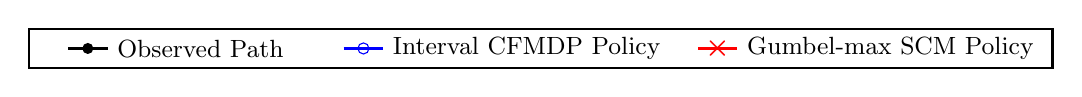
\begin{tikzpicture}[scale=1.0, every node/.style={scale=1.0}]
            \draw[thick, black] (-3, -0.25) rectangle (10, 0.25);
            %
            \draw[black, line width=1pt] (-2.5, 0.0) -- (-2,0.0);
            \fill[black] (-2.25,0.0) circle (2pt); %
            \node[right] at (-2,0.0) {\small Observed Path};
            
            %
            \draw[blue, line width=1pt] (1.0,0.0) -- (1.5,0.0);
            \node[draw=blue, circle, minimum size=4pt, inner sep=0pt] at (1.25,0.0) {}; %
            \node[right] at (1.5,0.0) {\small Interval CFMDP Policy};
            
            %
            \draw[red, line width=1pt] (5.5,0) -- (6,0);
            \node[red] at (5.75,0) {$\boldsymbol{\times}$}; %
            \node[right] at (6,0) {\small Gumbel-max SCM Policy};
        \end{tikzpicture}
    }\\
    %
    \subfigure[\footnotesize Lowest cumulative reward: Interval CFMDP ($312$), Gumbel-max SCM ($312$)]{%
        \resizebox{0.76\columnwidth}{!}{
             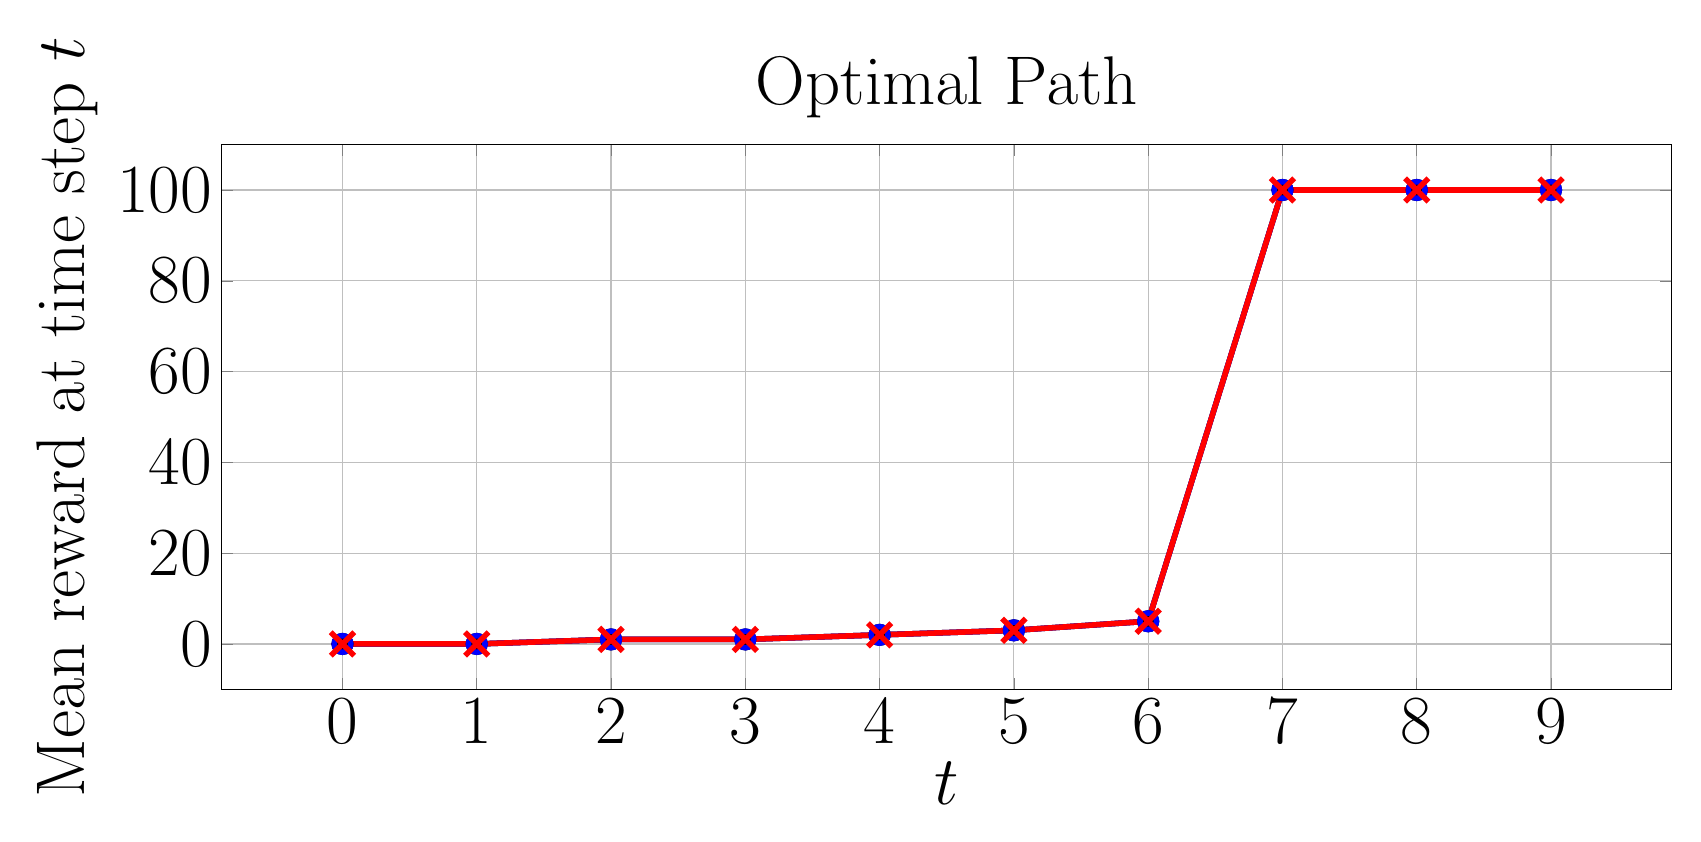
\begin{tikzpicture}
                \begin{axis}[
                    xlabel={$t$},
                    ylabel={Mean reward at time step $t$},
                    title={Optimal Path},
                    grid=both,
                    width=20cm, height=8.5cm,
                    every axis/.style={font=\Huge},
                    %
                ]
                \addplot[
                    color=black, %
                    mark=*, %
                    line width=2pt,
                    mark size=3pt,
                    error bars/.cd,
                    y dir=both, %
                    y explicit, %
                    error bar style={line width=1pt,solid},
                    error mark options={line width=1pt,mark size=4pt,rotate=90}
                ]
                coordinates {
                    (0, 0.0)  +- (0, 0.0)
                    (1, 0.0)  +- (0, 0.0) 
                    (2, 1.0)  +- (0, 0.0) 
                    (3, 1.0)  +- (0, 0.0)
                    (4, 2.0)  +- (0, 0.0)
                    (5, 3.0) +- (0, 0.0)
                    (6, 5.0) +- (0, 0.0)
                    (7, 100.0) +- (0, 0.0)
                    (8, 100.0) +- (0, 0.0)
                    (9, 100.0) +- (0, 0.0)
                };
                %
                \addplot[
                    color=blue, %
                    mark=o, %
                    line width=2pt,
                    mark size=3pt,
                    error bars/.cd,
                    y dir=both, %
                    y explicit, %
                    error bar style={line width=1pt,solid},
                    error mark options={line width=1pt,mark size=4pt,rotate=90}
                ]
                 coordinates {
                    (0, 0.0)  +- (0, 0.0)
                    (1, 0.0)  +- (0, 0.0) 
                    (2, 1.0)  +- (0, 0.0) 
                    (3, 1.0)  +- (0, 0.0)
                    (4, 2.0)  +- (0, 0.0)
                    (5, 3.0) +- (0, 0.0)
                    (6, 5.0) +- (0, 0.0)
                    (7, 100.0) +- (0, 0.0)
                    (8, 100.0) +- (0, 0.0)
                    (9, 100.0) +- (0, 0.0)
                };
                %
                \addplot[
                    color=red, %
                    mark=x, %
                    line width=2pt,
                    mark size=6pt,
                    error bars/.cd,
                    y dir=both, %
                    y explicit, %
                    error bar style={line width=1pt,solid},
                    error mark options={line width=1pt,mark size=4pt,rotate=90}
                ]
                coordinates {
                    (0, 0.0)  +- (0, 0.0)
                    (1, 0.0)  +- (0, 0.0) 
                    (2, 1.0)  +- (0, 0.0) 
                    (3, 1.0)  +- (0, 0.0)
                    (4, 2.0)  +- (0, 0.0)
                    (5, 3.0) +- (0, 0.0)
                    (6, 5.0) +- (0, 0.0)
                    (7, 100.0) +- (0, 0.0)
                    (8, 100.0) +- (0, 0.0)
                    (9, 100.0) +- (0, 0.0)
                };
                \end{axis}
            \end{tikzpicture}
         }
    }
    \hspace{1cm}
    \subfigure[\footnotesize Lowest cumulative reward: Interval CFMDP ($19$), Gumbel-max SCM ($-88$)]{%
         \resizebox{0.76\columnwidth}{!}{
            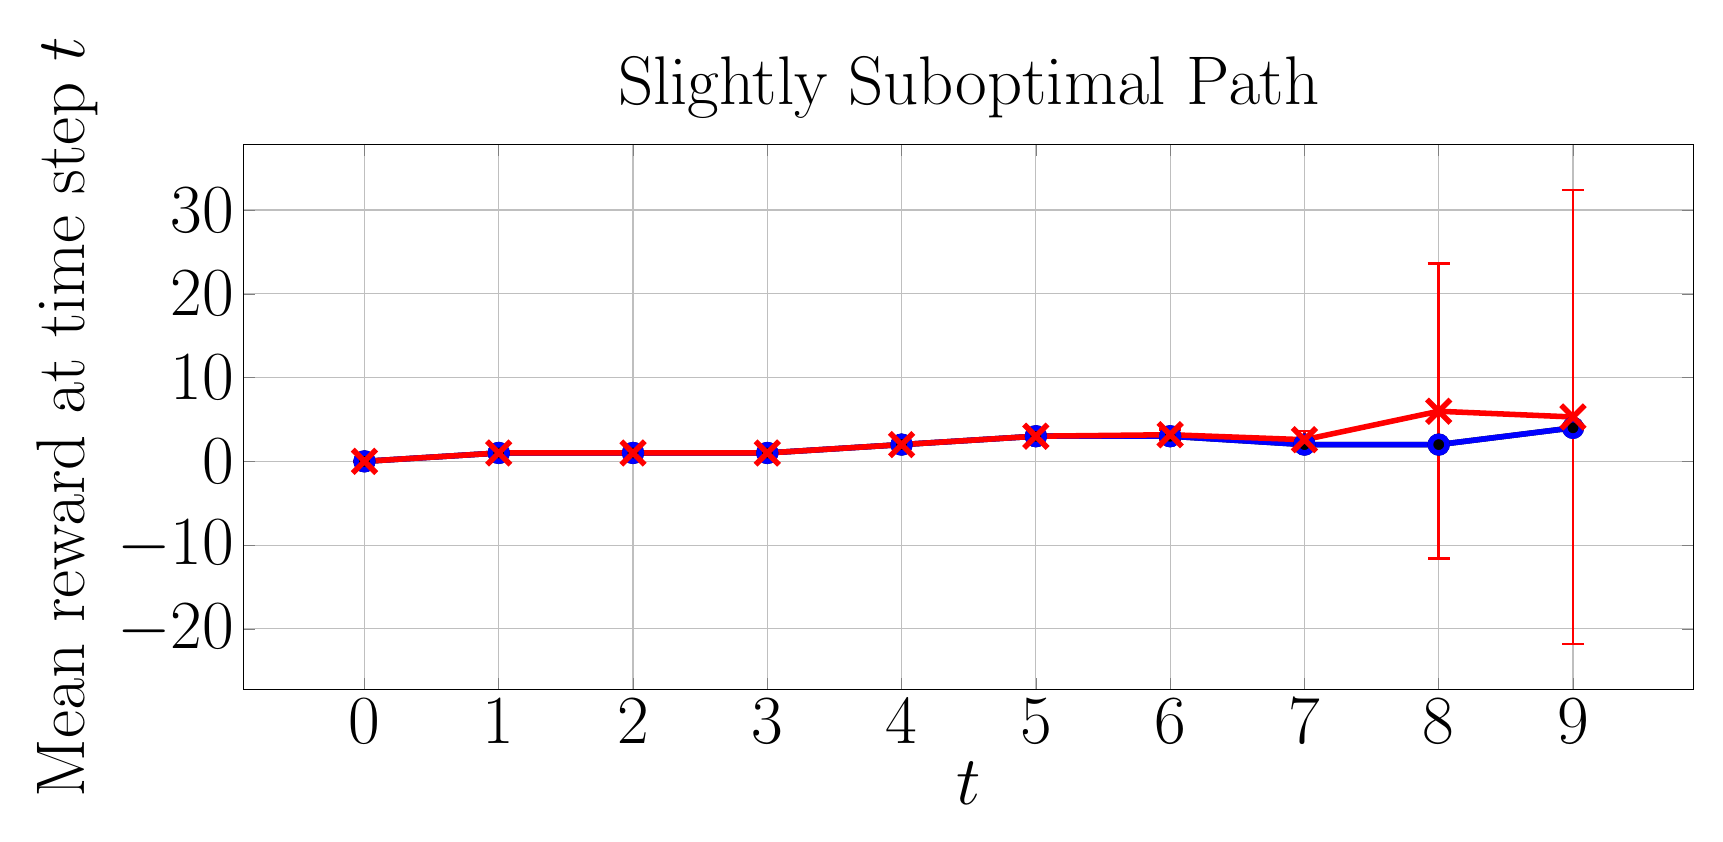
\begin{tikzpicture}
                \begin{axis}[
                    xlabel={$t$},
                    ylabel={Mean reward at time step $t$},
                    title={Slightly Suboptimal Path},
                    grid=both,
                    width=20cm, height=8.5cm,
                    every axis/.style={font=\Huge},
                    %
                ]
                \addplot[
                    color=black, %
                    mark=*, %
                    line width=2pt,
                    mark size=3pt,
                    error bars/.cd,
                    y dir=both, %
                    y explicit, %
                    error bar style={line width=1pt,solid},
                    error mark options={line width=1pt,mark size=4pt,rotate=90}
                ]
              coordinates {
                    (0, 0.0)  +- (0, 0.0)
                    (1, 1.0)  +- (0, 0.0) 
                    (2, 1.0)  +- (0, 0.0) 
                    (3, 1.0)  +- (0, 0.0)
                    (4, 2.0)  +- (0, 0.0)
                    (5, 3.0) +- (0, 0.0)
                    (6, 3.0) +- (0, 0.0)
                    (7, 2.0) +- (0, 0.0)
                    (8, 2.0) +- (0, 0.0)
                    (9, 4.0) +- (0, 0.0)
                };
                %
                \addplot[
                    color=blue, %
                    mark=o, %
                    line width=2pt,
                    mark size=3pt,
                    error bars/.cd,
                    y dir=both, %
                    y explicit, %
                    error bar style={line width=1pt,solid},
                    error mark options={line width=1pt,mark size=4pt,rotate=90}
                ]
              coordinates {
                    (0, 0.0)  +- (0, 0.0)
                    (1, 1.0)  +- (0, 0.0) 
                    (2, 1.0)  +- (0, 0.0) 
                    (3, 1.0)  +- (0, 0.0)
                    (4, 2.0)  +- (0, 0.0)
                    (5, 3.0) +- (0, 0.0)
                    (6, 3.0) +- (0, 0.0)
                    (7, 2.0) +- (0, 0.0)
                    (8, 2.0) +- (0, 0.0)
                    (9, 4.0) +- (0, 0.0)
                };
                %
                \addplot[
                    color=red, %
                    mark=x, %
                    line width=2pt,
                    mark size=6pt,
                    error bars/.cd,
                    y dir=both, %
                    y explicit, %
                    error bar style={line width=1pt,solid},
                    error mark options={line width=1pt,mark size=4pt,rotate=90}
                ]
                coordinates {
                    (0, 0.0)  +- (0, 0.0)
                    (1, 1.0)  +- (0, 0.0) 
                    (2, 1.0)  +- (0, 0.0) 
                    (3, 1.0)  +- (0, 0.0)
                    (4, 2.0)  += (0, 0.0)
                    (5, 3.0)  += (0, 0.0)
                    (6, 3.17847) += (0, 0.62606746) -= (0, 0.62606746)
                    (7, 2.5832885) += (0, 1.04598233) -= (0, 1.04598233)
                    (8, 5.978909) += (0, 17.60137623) -= (0, 17.60137623)
                    (9, 5.297059) += (0, 27.09227512) -= (0, 27.09227512)
                };
                \end{axis}
            \end{tikzpicture}
         }
    }\\[-1.5pt]
    \subfigure[\footnotesize Lowest cumulative reward: Interval CFMDP ($14$), Gumbel-max SCM ($-598$)]{%
         \resizebox{0.76\columnwidth}{!}{
             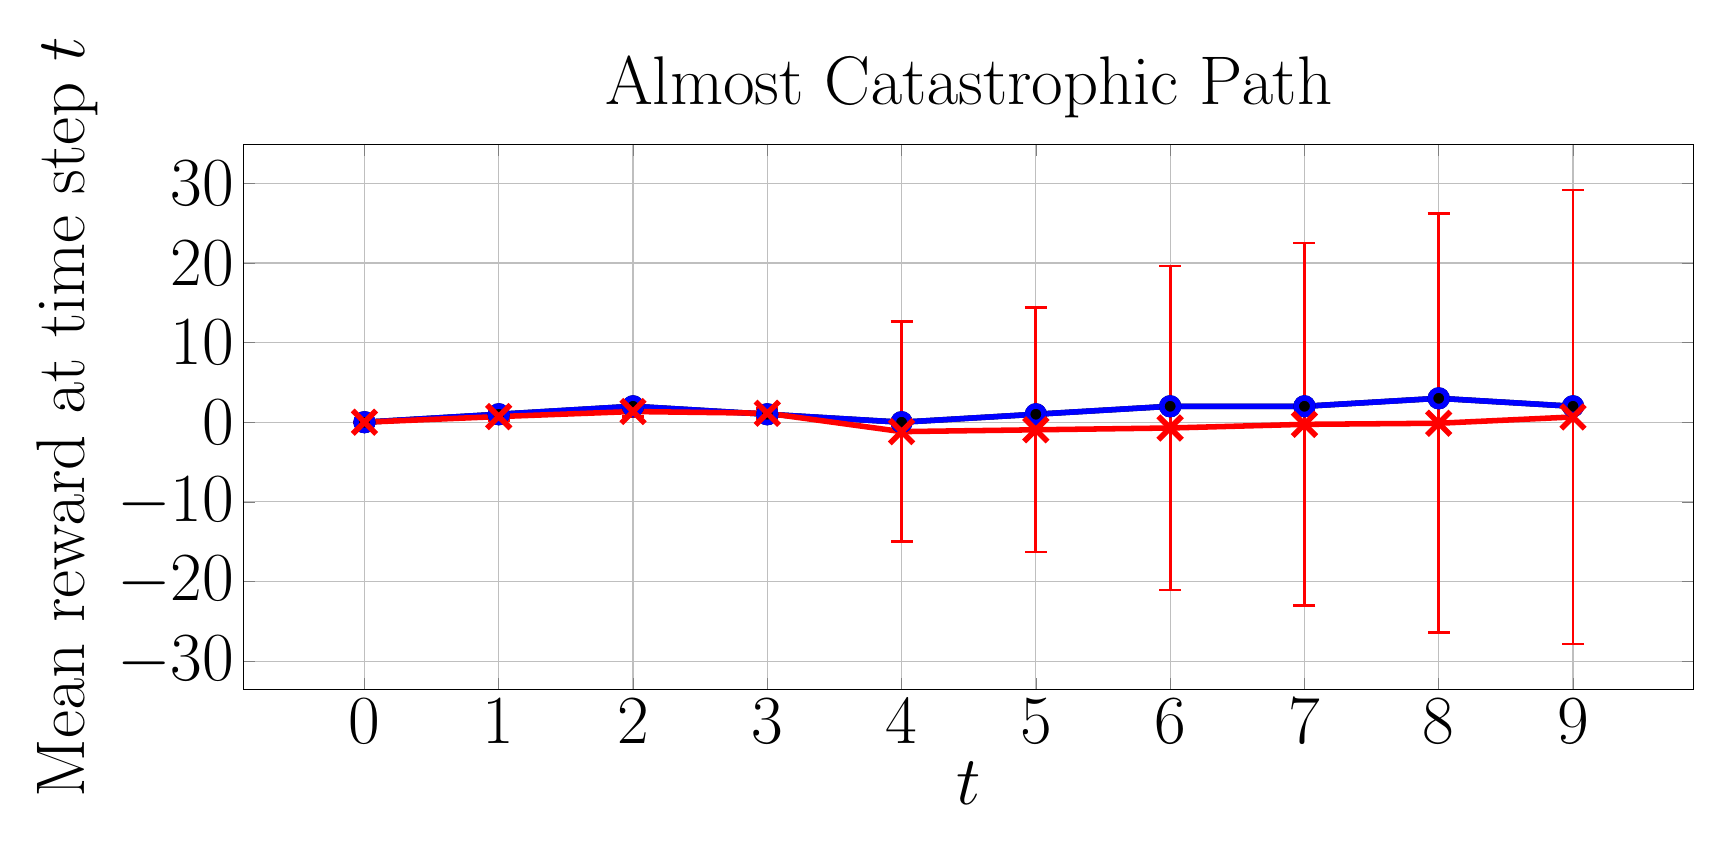
\begin{tikzpicture}
                \begin{axis}[
                    xlabel={$t$},
                    ylabel={Mean reward at time step $t$},
                    title={Almost Catastrophic Path},
                    grid=both,
                    width=20cm, height=8.5cm,
                    every axis/.style={font=\Huge},
                    %
                ]
                \addplot[
                    color=black, %
                    mark=*, %
                    line width=2pt,
                    mark size=3pt,
                    error bars/.cd,
                    y dir=both, %
                    y explicit, %
                    error bar style={line width=1pt,solid},
                    error mark options={line width=1pt,mark size=4pt,rotate=90}
                ]
                coordinates {
                    (0, 0.0)  +- (0, 0.0)
                    (1, 1.0)  +- (0, 0.0) 
                    (2, 2.0)  +- (0, 0.0) 
                    (3, 1.0)  +- (0, 0.0)
                    (4, 0.0)  +- (0, 0.0)
                    (5, 1.0) +- (0, 0.0)
                    (6, 2.0) +- (0, 0.0)
                    (7, 2.0) +- (0, 0.0)
                    (8, 3.0) +- (0, 0.0)
                    (9, 2.0) +- (0, 0.0)
                };
                %
                \addplot[
                    color=blue, %
                    mark=o, %
                    line width=2pt,
                    mark size=3pt,
                    error bars/.cd,
                    y dir=both, %
                    y explicit, %
                    error bar style={line width=1pt,solid},
                    error mark options={line width=1pt,mark size=4pt,rotate=90}
                ]
                coordinates {
                    (0, 0.0)  +- (0, 0.0)
                    (1, 1.0)  +- (0, 0.0) 
                    (2, 2.0)  +- (0, 0.0) 
                    (3, 1.0)  +- (0, 0.0)
                    (4, 0.0)  +- (0, 0.0)
                    (5, 1.0) +- (0, 0.0)
                    (6, 2.0) +- (0, 0.0)
                    (7, 2.0) +- (0, 0.0)
                    (8, 3.0) +- (0, 0.0)
                    (9, 2.0) +- (0, 0.0)
                };
                %
                \addplot[
                    color=red, %
                    mark=x, %
                    line width=2pt,
                    mark size=6pt,
                    error bars/.cd,
                    y dir=both, %
                    y explicit, %
                    error bar style={line width=1pt,solid},
                    error mark options={line width=1pt,mark size=4pt,rotate=90}
                ]
                coordinates {
                    (0, 0.0)  +- (0, 0.0)
                    (1, 0.7065655)  +- (0, 0.4553358) 
                    (2, 1.341673)  +- (0, 0.67091621) 
                    (3, 1.122926)  +- (0, 0.61281824)
                    (4, -1.1821935)  +- (0, 13.82444042)
                    (5, -0.952399)  +- (0, 15.35195457)
                    (6, -0.72672) +- (0, 20.33508414)
                    (7, -0.268983) +- (0, 22.77861454)
                    (8, -0.1310835) +- (0, 26.31013314)
                    (9, 0.65806) +- (0, 28.50670214)
                };
                %
            %
            %
            %
            %
            %
            %
            %
            %
            %
            %
            %
            %
            %
            %
            %
            %
            %
            %
                \end{axis}
            \end{tikzpicture}
         }
    }
    \hspace{1cm}
    \subfigure[\footnotesize Lowest cumulative reward: Interval CFMDP ($-698$), Gumbel-max SCM ($-698$)]{%
         \resizebox{0.76\columnwidth}{!}{
            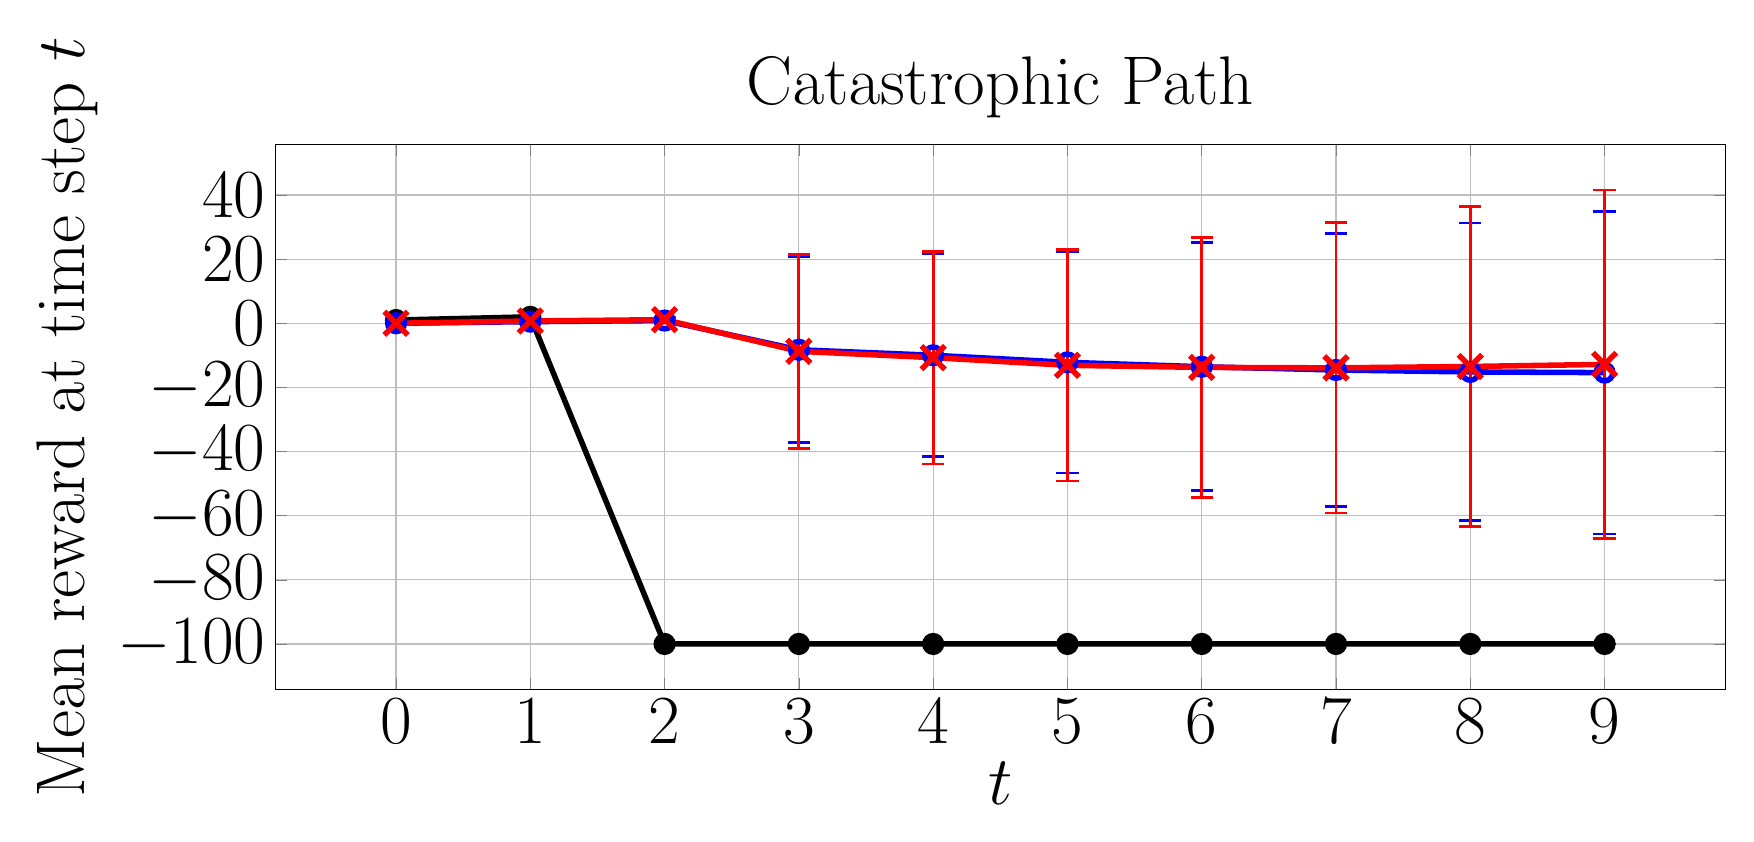
\begin{tikzpicture}
                \begin{axis}[
                    xlabel={$t$},
                    ylabel={Mean reward at time step $t$},
                    title={Catastrophic Path},
                    grid=both,
                    width=20cm, height=8.5cm,
                    every axis/.style={font=\Huge},
                    %
                ]
                \addplot[
                    color=black, %
                    mark=*, %
                    line width=2pt,
                    mark size=3pt,
                    error bars/.cd,
                    y dir=both, %
                    y explicit, %
                    error bar style={line width=1pt,solid},
                    error mark options={line width=1pt,mark size=4pt,rotate=90}
                ]
                coordinates {
                    (0, 1.0)  +- (0, 0.0)
                    (1, 2.0)  +- (0, 0.0) 
                    (2, -100.0)  +- (0, 0.0) 
                    (3, -100.0)  +- (0, 0.0)
                    (4, -100.0)  +- (0, 0.0)
                    (5, -100.0) +- (0, 0.0)
                    (6, -100.0) +- (0, 0.0)
                    (7, -100.0) +- (0, 0.0)
                    (8, -100.0) +- (0, 0.0)
                    (9, -100.0) +- (0, 0.0)
                };
                %
                \addplot[
                    color=blue, %
                    mark=o, %
                    line width=2pt,
                    mark size=3pt,
                    error bars/.cd,
                    y dir=both, %
                    y explicit, %
                    error bar style={line width=1pt,solid},
                    error mark options={line width=1pt,mark size=4pt,rotate=90}
                ]
                coordinates {
                    (0, 0.0)  +- (0, 0.0)
                    (1, 0.504814)  +- (0, 0.49997682) 
                    (2, 0.8439835)  +- (0, 0.76831917) 
                    (3, -8.2709165)  +- (0, 28.93656754)
                    (4, -9.981082)  +- (0, 31.66825363)
                    (5, -12.1776325) +- (0, 34.53463233)
                    (6, -13.556076) +- (0, 38.62845372)
                    (7, -14.574418) +- (0, 42.49603359)
                    (8, -15.1757075) +- (0, 46.41913968)
                    (9, -15.3900395) +- (0, 50.33563368)
                };
                %
                \addplot[
                    color=red, %
                    mark=x, %
                    line width=2pt,
                    mark size=6pt,
                    error bars/.cd,
                    y dir=both, %
                    y explicit, %
                    error bar style={line width=1pt,solid},
                    error mark options={line width=1pt,mark size=4pt,rotate=90}
                ]
                coordinates {
                    (0, 0.0)  +- (0, 0.0)
                    (1, 0.701873)  +- (0, 0.45743556) 
                    (2, 1.1227805)  +- (0, 0.73433129) 
                    (3, -8.7503255)  +- (0, 30.30257976)
                    (4, -10.722092)  +- (0, 33.17618589)
                    (5, -13.10721)  +- (0, 36.0648089)
                    (6, -13.7631645) +- (0, 40.56553451)
                    (7, -13.909043) +- (0, 45.23829402)
                    (8, -13.472517) +- (0, 49.96270296)
                    (9, -12.8278835) +- (0, 54.38618735)
                };
                %
            %
            %
            %
            %
            %
            %
            %
            %
            %
            %
            %
            %
            %
            %
            %
            %
            %
            %
                \end{axis}
            \end{tikzpicture}
         }
    }
    \caption{Average instant reward of CF paths induced by policies on GridWorld $p=0.4$.}
    \label{fig: reward p=0.4}
\end{figure*}

\subsection{Experimental Setup}
To compare policy performance, we measure the average rewards of counterfactual paths induced by our policy and the Gumbel-max policy by uniformly sampling $200$ counterfactual MDPs from the ICFMDP and generating $10,000$ counterfactual paths over each sampled CFMDP. \jl{Since the interval CFMDP depends on the observed path, we select $4$  paths of varying optimality to evaluate how the observed path impacts the performance of both policies: an optimal path, a slightly suboptimal path that could reach the optimal reward with a few changes, a catastrophic path that enters a catastrophic, terminal state with low reward, and an almost catastrophic path that was close to entering a catastrophic state.} When measuring the average probability bound widths and execution time needed to generate the ICFMDPs, we averaged over $20$ randomly generated observed paths
\footnote{Further training details are provided in Appendix \ref{app: training details}, and the code is provided at \href{https://github.com/ddv-lab/robust-cf-inference-in-MDPs}{https://github.com/ddv-lab/robust-cf-inference-in-MDPs}
%
%
.}.

\subsection{GridWorld}
\jl{The GridWorld MDP is a $4 \times 4$ grid where an agent must navigate from the top-left corner to the goal state in the bottom-right corner, avoiding a dangerous terminal state in the centre. At each time step, the agent can move up, down, left, or right, but there is a small probability (controlled by hyper-parameter $p$) of moving in an unintended direction. As the agent nears the goal, the reward for each state increases, culminating in a reward of $+100$ for reaching the goal. Entering the dangerous state results in a penalty of $-100$. We use two versions of GridWorld: a less stochastic version with $p=0.9$ (i.e., $90$\% chance of moving in the chosen direction) and a more stochastic version with $p=0.4$.}

\paragraph{GridWorld ($p=0.9$)}
When $p=0.9$, the counterfactual probability bounds are typically narrow (see Table \ref{tab:nonzero_probs} for average measurements). Consequently, as shown in Figure \ref{fig: reward p=0.9}, both policies are nearly identical and perform similarly well across the optimal, slightly suboptimal, and catastrophic paths.
%
However, for the almost catastrophic path, the interval CFMDP path is more conservative and follows the observed path more closely (as this is where the probability bounds are narrowest), which typically requires one additional step to reach the goal state than the Gumbel-max SCM policy.
%

\paragraph{GridWorld ($p=0.4$)}
\jl{When $p=0.4$, the GridWorld environment becomes more uncertain, increasing the risk of entering the dangerous state even if correct actions are chosen. Thus, as shown in Figure \ref{fig: reward p=0.4}, the interval CFMDP policy adopts a more conservative approach, avoiding deviation from the observed policy if it cannot guarantee higher counterfactual rewards (see the slightly suboptimal and almost catastrophic paths), whereas the Gumbel-max SCM is inconsistent: it can yield higher rewards, but also much lower rewards, reflected in the wide error bars.} For the catastrophic path, both policies must deviate from the observed path to achieve a higher reward and, in this case, perform similarly.
%
%
%
%
\subsection{Sepsis}
The Sepsis MDP \citep{oberst2019counterfactual} simulates trajectories of Sepsis patients. Each state consists of four vital signs (heart rate, blood pressure, oxygen concentration, and glucose levels), categorised as low, normal, or high.
and three treatments that can be toggled on/off at each time step (8 actions in total). Unlike \citet{oberst2019counterfactual}, we scale rewards based on the number of out-of-range vital signs, between $-1000$ (patient dies) and $1000$ (patient discharged). \jl{Like the GridWorld $p=0.4$ experiment, the Sepsis MDP is highly uncertain, as many states are equally likely to lead to optimal and poor outcomes. Thus, as shown in Figure \ref{fig: reward sepsis}, both policies follow the observed optimal and almost catastrophic paths to guarantee rewards are no worse than the observation.} However, improving the catastrophic path requires deviating from the observation. Here, the Gumbel-max SCM policy, on average, performs better than the interval CFMDP policy. But, since both policies have lower bounds clipped at $-1000$, neither policy reliably improves over the observation. In contrast, for the slightly suboptimal path, the interval CFMDP policy performs significantly better, shown by its higher lower bounds. 
Moreover, in these two cases, the worst-case counterfactual path generated by the interval CFMDP policy is better than that of the Gumbel-max SCM policy,
indicating its greater robustness.
%
\begin{figure*}
    \centering
     \resizebox{0.6\textwidth}{!}{
        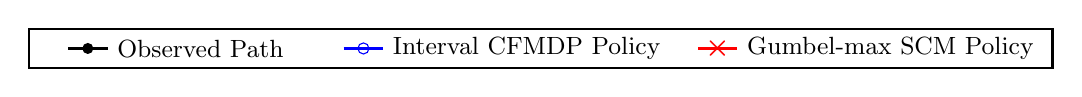
\begin{tikzpicture}[scale=1.0, every node/.style={scale=1.0}]
            \draw[thick, black] (-3, -0.25) rectangle (10, 0.25);
            %
            \draw[black, line width=1pt] (-2.5, 0.0) -- (-2,0.0);
            \fill[black] (-2.25,0.0) circle (2pt); %
            \node[right] at (-2,0.0) {\small Observed Path};
            
            %
            \draw[blue, line width=1pt] (1.0,0.0) -- (1.5,0.0);
            \node[draw=blue, circle, minimum size=4pt, inner sep=0pt] at (1.25,0.0) {}; %
            \node[right] at (1.5,0.0) {\small Interval CFMDP Policy};
            
            %
            \draw[red, line width=1pt] (5.5,0) -- (6,0);
            \node[red] at (5.75,0) {$\boldsymbol{\times}$}; %
            \node[right] at (6,0) {\small Gumbel-max SCM Policy};
        \end{tikzpicture}
    }\\
    \subfigure[\footnotesize Lowest cumulative reward: Interval CFMDP ($8000$), Gumbel-max SCM ($8000$)]{%
         \resizebox{0.76\columnwidth}{!}{
             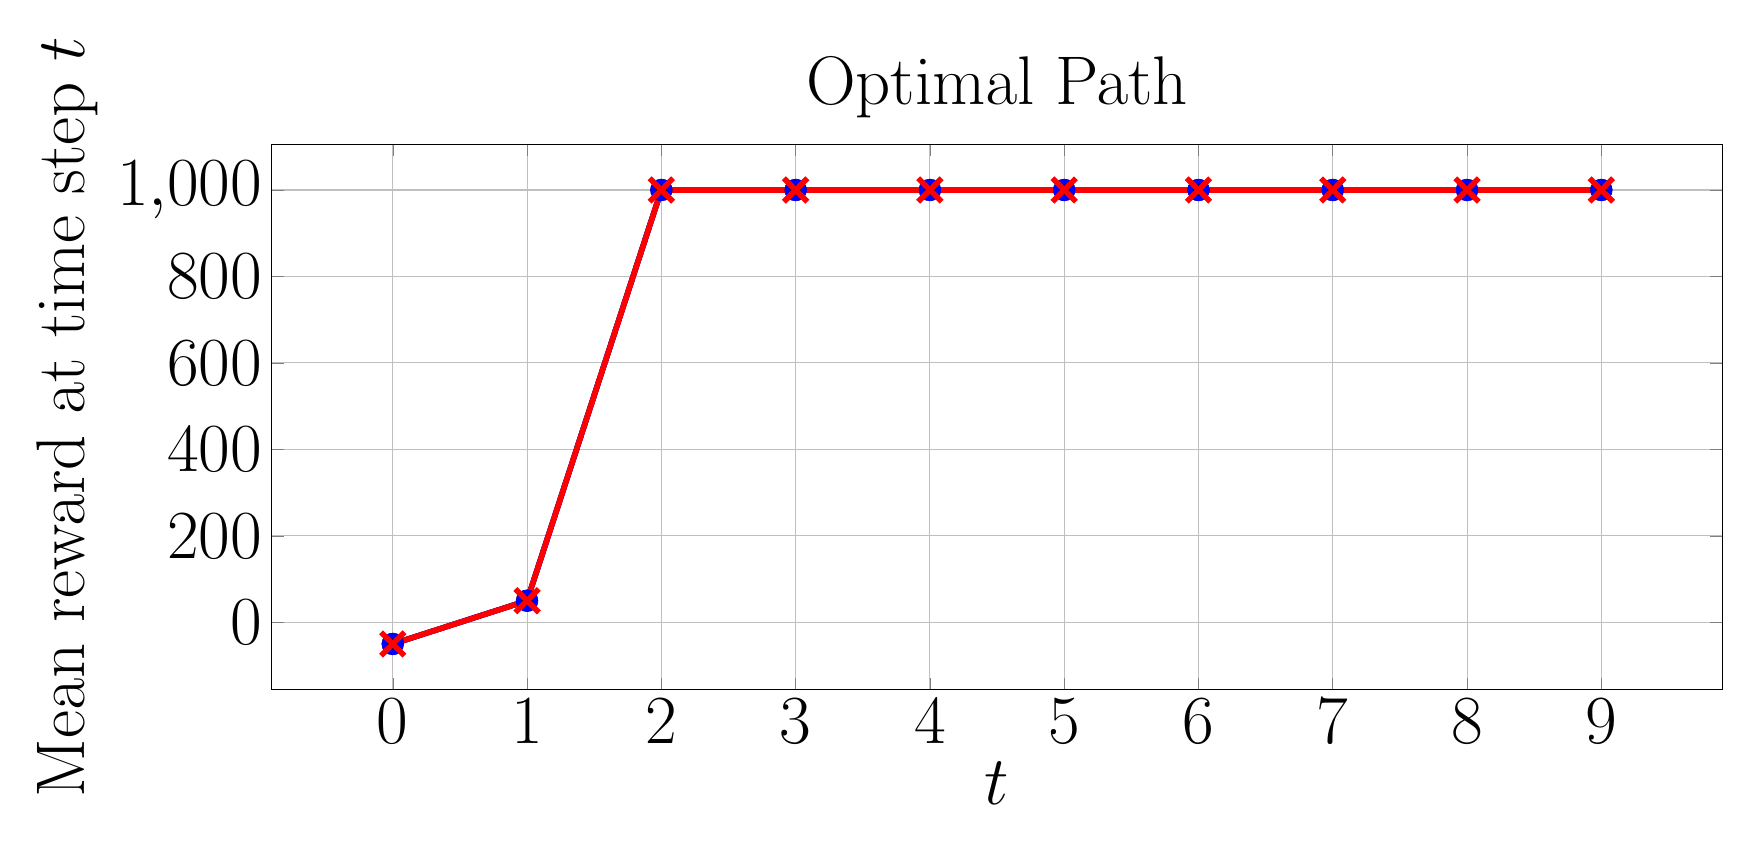
\begin{tikzpicture}
                \begin{axis}[
                    xlabel={$t$},
                    ylabel={Mean reward at time step $t$},
                    title={Optimal Path},
                    grid=both,
                    width=20cm, height=8.5cm,
                    every axis/.style={font=\Huge},
                    %
                ]
                \addplot[
                    color=black, %
                    mark=*, %
                    line width=2pt,
                    mark size=3pt,
                ]
                coordinates {
                    (0, -50.0)
                    (1, 50.0)
                    (2, 1000.0)
                    (3, 1000.0)
                    (4, 1000.0)
                    (5, 1000.0)
                    (6, 1000.0)
                    (7, 1000.0)
                    (8, 1000.0)
                    (9, 1000.0)
                };
                %
                \addplot[
                    color=blue, %
                    mark=o, %
                    line width=2pt,
                    mark size=3pt,
                    error bars/.cd,
                    y dir=both, %
                    y explicit, %
                    error bar style={line width=1pt,solid},
                    error mark options={line width=1pt,mark size=4pt,rotate=90}
                ]
                coordinates {
                    (0, -50.0)  +- (0, 0.0)
                    (1, 50.0)  +- (0, 0.0) 
                    (2, 1000.0)  +- (0, 0.0) 
                    (3, 1000.0)  +- (0, 0.0)
                    (4, 1000.0)  +- (0, 0.0)
                    (5, 1000.0) +- (0, 0.0)
                    (6, 1000.0) +- (0, 0.0)
                    (7, 1000.0) +- (0, 0.0)
                    (8, 1000.0) +- (0, 0.0)
                    (9, 1000.0) +- (0, 0.0)
                };
                %
                \addplot[
                    color=red, %
                    mark=x, %
                    line width=2pt,
                    mark size=6pt,
                    error bars/.cd,
                    y dir=both, %
                    y explicit, %
                    error bar style={line width=1pt,solid},
                    error mark options={line width=1pt,mark size=4pt,rotate=90}
                ]
                coordinates {
                    (0, -50.0)  +- (0, 0.0)
                    (1, 50.0)  +- (0, 0.0) 
                    (2, 1000.0)  +- (0, 0.0) 
                    (3, 1000.0)  +- (0, 0.0)
                    (4, 1000.0)  +- (0, 0.0)
                    (5, 1000.0) +- (0, 0.0)
                    (6, 1000.0) +- (0, 0.0)
                    (7, 1000.0) +- (0, 0.0)
                    (8, 1000.0) +- (0, 0.0)
                    (9, 1000.0) +- (0, 0.0)
                };
                %
                \end{axis}
            \end{tikzpicture}
         }
    }
    \hspace{1cm}
    \subfigure[\footnotesize Lowest cumulative reward: Interval CFMDP ($-5980$), Gumbel-max SCM ($-8000$)]{%
         \resizebox{0.76\columnwidth}{!}{
            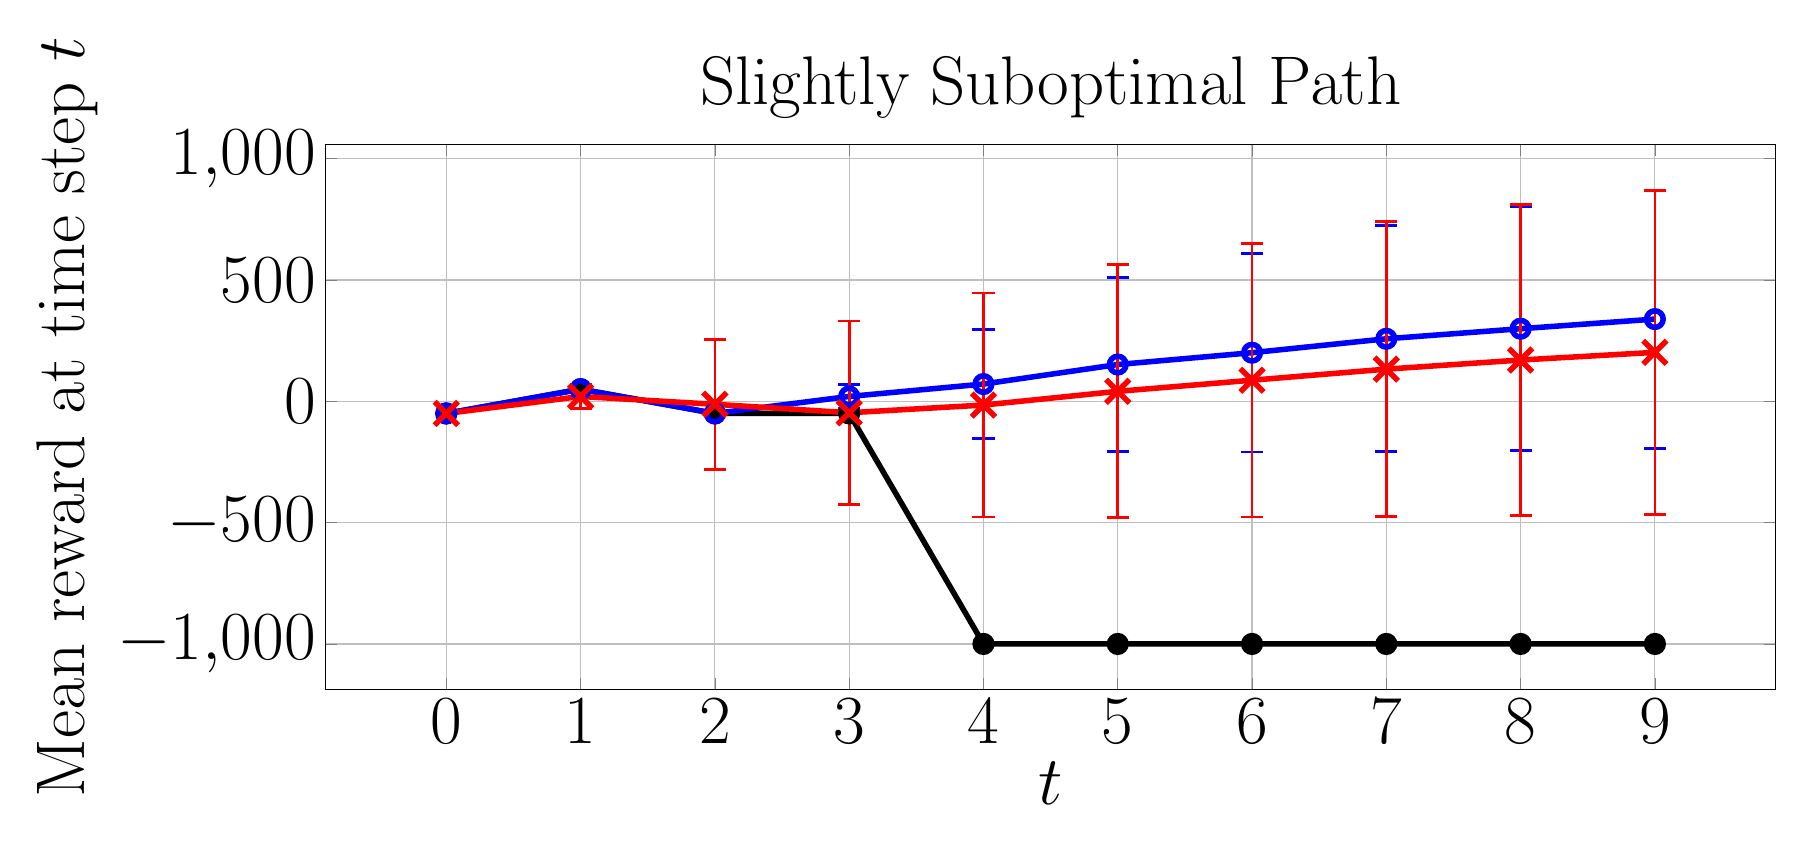
\begin{tikzpicture}
                \begin{axis}[
                    xlabel={$t$},
                    ylabel={Mean reward at time step $t$},
                    title={Slightly Suboptimal Path},
                    grid=both,
                    width=20cm, height=8.5cm,
                    every axis/.style={font=\Huge},
                    %
                ]
               \addplot[
                    color=black, %
                    mark=*, %
                    line width=2pt,
                    mark size=3pt,
                ]
                coordinates {
                    (0, -50.0)
                    (1, 50.0)
                    (2, -50.0)
                    (3, -50.0)
                    (4, -1000.0)
                    (5, -1000.0)
                    (6, -1000.0)
                    (7, -1000.0)
                    (8, -1000.0)
                    (9, -1000.0)
                };
                %
                \addplot[
                    color=blue, %
                    mark=o, %
                    line width=2pt,
                    mark size=3pt,
                    error bars/.cd,
                    y dir=both, %
                    y explicit, %
                    error bar style={line width=1pt,solid},
                    error mark options={line width=1pt,mark size=4pt,rotate=90}
                ]
                coordinates {
                    (0, -50.0)  +- (0, 0.0)
                    (1, 50.0)  +- (0, 0.0) 
                    (2, -50.0)  +- (0, 0.0) 
                    (3, 20.0631)  +- (0, 49.97539413)
                    (4, 71.206585)  +- (0, 226.02033693)
                    (5, 151.60797) +- (0, 359.23292559)
                    (6, 200.40593) +- (0, 408.86185176)
                    (7, 257.77948) +- (0, 466.10372804)
                    (8, 299.237465) +- (0, 501.82579506)
                    (9, 338.9129) +- (0, 532.06124996)
                };
                %
                \addplot[
                    color=red, %
                    mark=x, %
                    line width=2pt,
                    mark size=6pt,
                    error bars/.cd,
                    y dir=both, %
                    y explicit, %
                    error bar style={line width=1pt,solid},
                    error mark options={line width=1pt,mark size=4pt,rotate=90}
                ]
                coordinates {
                    (0, -50.0)  +- (0, 0.0)
                    (1, 20.00736)  +- (0, 49.99786741) 
                    (2, -12.282865)  +- (0, 267.598755) 
                    (3, -47.125995)  +- (0, 378.41755832)
                    (4, -15.381965)  +- (0, 461.77616558)
                    (5, 41.15459) +- (0, 521.53189262)
                    (6, 87.01595) +- (0, 564.22243126 )
                    (7, 132.62376) +- (0, 607.31338037)
                    (8, 170.168145) +- (0, 641.48013693)
                    (9, 201.813135) +- (0, 667.29441777)
                };
                %
                %
                %
                %
                %
                %
                %
                %
                %
                %
                %
                %
                %
                %
                %
                %
                %
                %
                %
                \end{axis}
            \end{tikzpicture}
         }
    }\\[-1.5pt]
    \subfigure[\footnotesize Lowest cumulative reward: Interval CFMDP ($100$), Gumbel-max SCM ($100$)]{%
         \resizebox{0.76\columnwidth}{!}{
             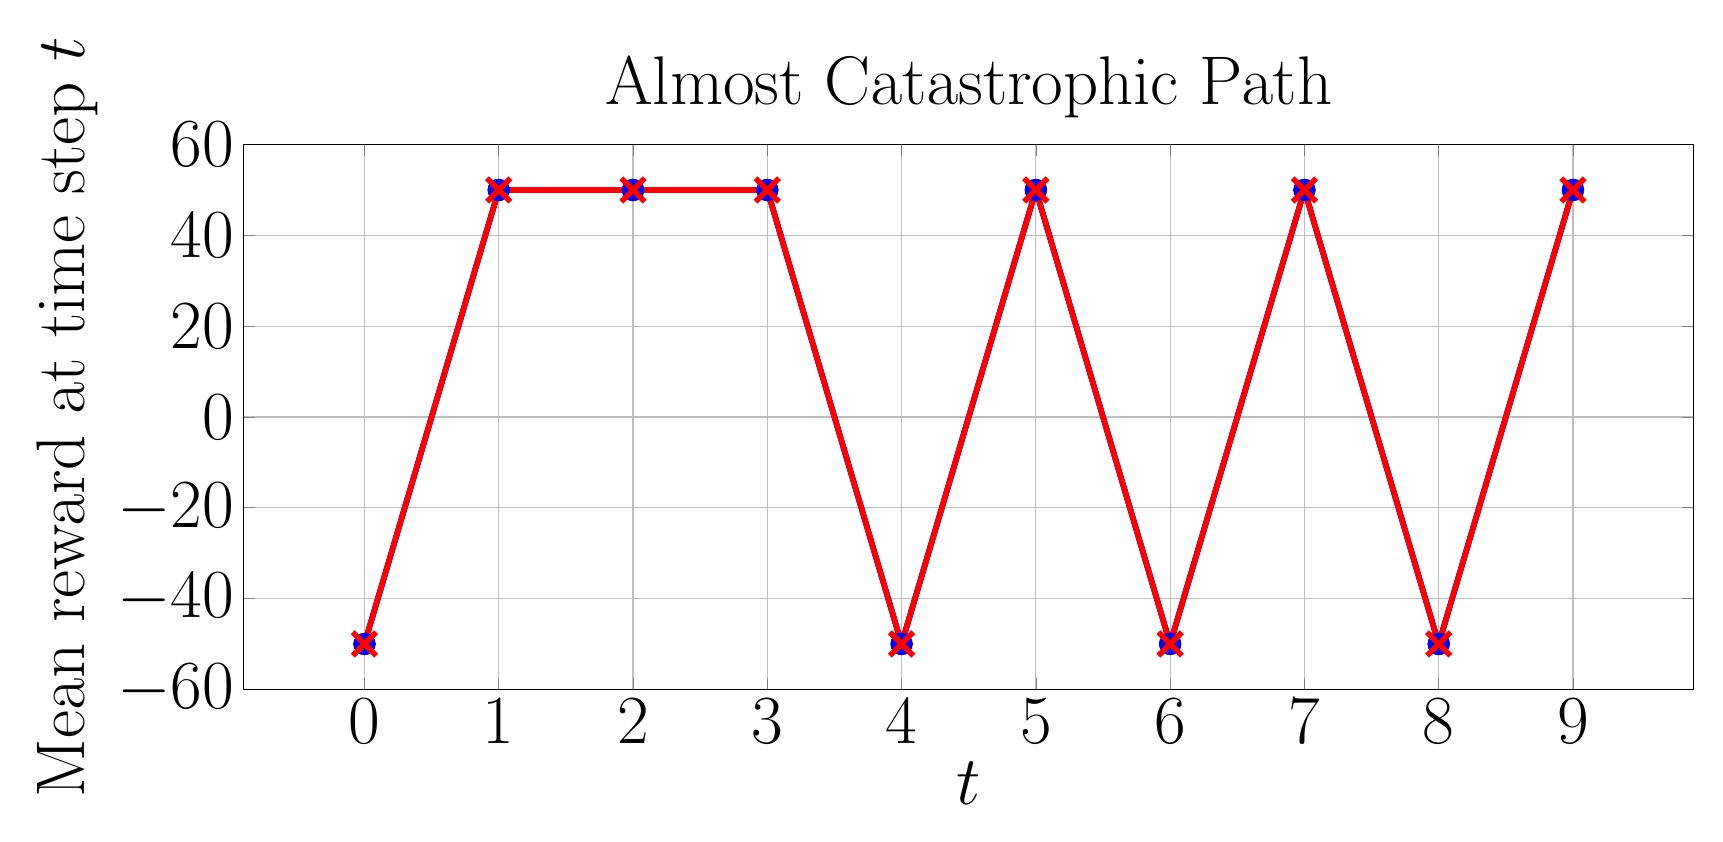
\begin{tikzpicture}
                \begin{axis}[
                    xlabel={$t$},
                    ylabel={Mean reward at time step $t$},
                    title={Almost Catastrophic Path},
                    grid=both,
                    every axis/.style={font=\Huge},
                    width=20cm, height=8.5cm,
                    %
                ]
               \addplot[
                    color=black, %
                    mark=*, %
                    line width=2pt,
                    mark size=3pt,
                ]
                coordinates {
                    (0, -50.0)
                    (1, 50.0)
                    (2, 50.0)
                    (3, 50.0)
                    (4, -50.0)
                    (5, 50.0)
                    (6, -50.0)
                    (7, 50.0)
                    (8, -50.0)
                    (9, 50.0)
                };
                %
                %
                \addplot[
                    color=blue, %
                    mark=o, %
                    line width=2pt,
                    mark size=3pt,
                    error bars/.cd,
                    y dir=both, %
                    y explicit, %
                    error bar style={line width=1pt,solid},
                    error mark options={line width=1pt,mark size=4pt,rotate=90}
                ]
                coordinates {
                    (0, -50.0)  +- (0, 0.0)
                    (1, 50.0)  +- (0, 0.0) 
                    (2, 50.0)  +- (0, 0.0) 
                    (3, 50.0)  +- (0, 0.0)
                    (4, -50.0)  +- (0, 0.0)
                    (5, 50.0) +- (0, 0.0)
                    (6, -50.0) +- (0, 0.0)
                    (7, 50.0) +- (0, 0.0)
                    (8, -50.0) +- (0, 0.0)
                    (9, 50.0) +- (0, 0.0)
                };
                %
                \addplot[
                    color=red, %
                    mark=x, %
                    line width=2pt,
                    mark size=6pt,
                    error bars/.cd,
                    y dir=both, %
                    y explicit, %
                    error bar style={line width=1pt,solid},
                    error mark options={line width=1pt,mark size=4pt,rotate=90}
                ]
                coordinates {
                    (0, -50.0)  +- (0, 0.0)
                    (1, 50.0)  +- (0, 0.0) 
                    (2, 50.0)  +- (0, 0.0) 
                    (3, 50.0)  +- (0, 0.0)
                    (4, -50.0)  +- (0, 0.0)
                    (5, 50.0) +- (0, 0.0)
                    (6, -50.0) +- (0, 0.0)
                    (7, 50.0) +- (0, 0.0)
                    (8, -50.0) +- (0, 0.0)
                    (9, 50.0) +- (0, 0.0)
                };
                %
                %
                %
                %
                %
                %
                %
                %
                %
                %
                %
                %
                %
                %
                %
                %
                %
                %
                %
                \end{axis}
            \end{tikzpicture}
         }
    }
    \hspace{1cm}
    \subfigure[\footnotesize Lowest cumulative reward: Interval CFMDP ($-7150$), Gumbel-max SCM ($-9050$)]{%
         \resizebox{0.76\columnwidth}{!}{
            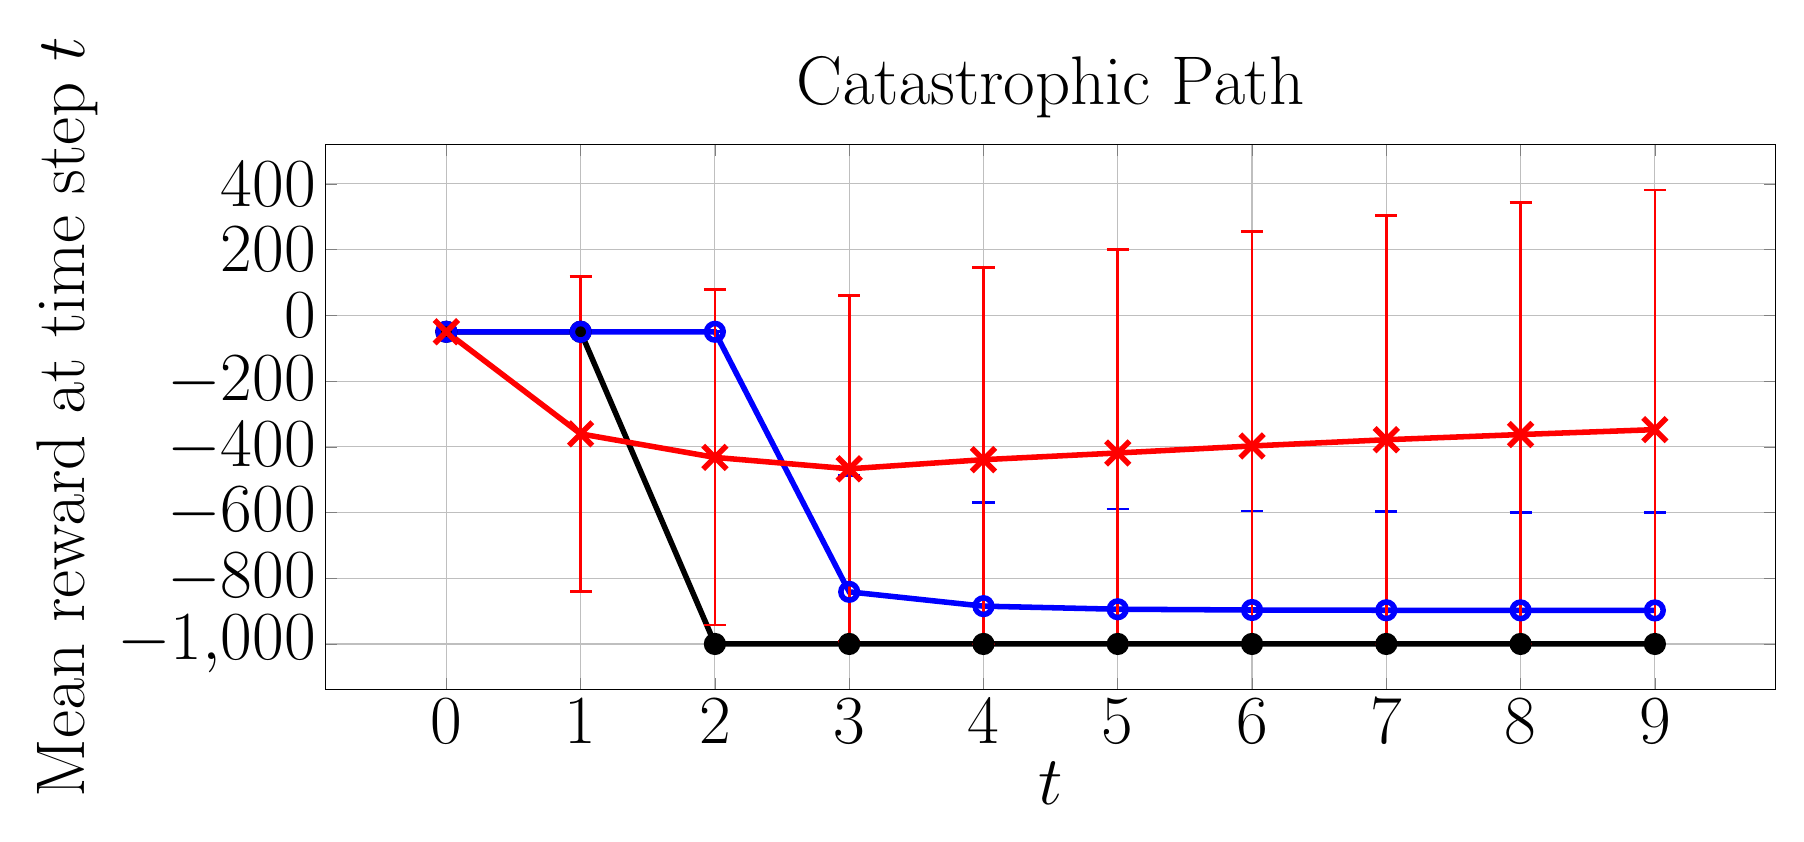
\begin{tikzpicture}
                \begin{axis}[
                    xlabel={$t$},
                    ylabel={Mean reward at time step $t$},
                    title={Catastrophic Path},
                    grid=both,
                    width=20cm, height=8.5cm,
                    every axis/.style={font=\Huge},
                    %
                ]
               \addplot[
                    color=black, %
                    mark=*, %
                    line width=2pt,
                    mark size=3pt,
                ]
                coordinates {
                    (0, -50.0)
                    (1, -50.0)
                    (2, -1000.0)
                    (3, -1000.0)
                    (4, -1000.0)
                    (5, -1000.0)
                    (6, -1000.0)
                    (7, -1000.0)
                    (8, -1000.0)
                    (9, -1000.0)
                };
                %
                %
                \addplot[
                    color=blue, %
                    mark=o, %
                    line width=2pt,
                    mark size=3pt,
                    error bars/.cd,
                    y dir=both, %
                    y explicit, %
                    error bar style={line width=1pt,solid},
                    error mark options={line width=1pt,mark size=4pt,rotate=90}
                ]
                coordinates {
                    (0, -50.0)  +- (0, 0.0)
                    (1, -50.0)  +- (0, 0.0) 
                    (2, -50.0)  +- (0, 0.0) 
                    (3, -841.440725)  += (0, 354.24605512) -= (0, 158.559275)
                    (4, -884.98225)  += (0, 315.37519669) -= (0, 115.01775)
                    (5, -894.330425) += (0, 304.88572805) -= (0, 105.669575)
                    (6, -896.696175) += (0, 301.19954514) -= (0, 103.303825)
                    (7, -897.4635) += (0, 299.61791279) -= (0, 102.5365)
                    (8, -897.77595) += (0, 298.80392585) -= (0, 102.22405)
                    (9, -897.942975) += (0, 298.32920557) -= (0, 102.057025)
                };
                %
                \addplot[
                    color=red, %
                    mark=x, %
                    line width=2pt,
                    mark size=6pt,
                    error bars/.cd,
                    y dir=both, %
                    y explicit, %
                    error bar style={line width=1pt,solid},
                    error mark options={line width=1pt,mark size=4pt,rotate=90}
                ]
            coordinates {
                    (0, -50.0)  +- (0, 0.0)
                    (1, -360.675265)  +- (0, 479.39812699) 
                    (2, -432.27629)  +- (0, 510.38620897) 
                    (3, -467.029545)  += (0, 526.36009628) -= (0, 526.36009628)
                    (4, -439.17429)  += (0, 583.96638919) -= (0, 560.82571)
                    (5, -418.82704) += (0, 618.43027478) -= (0, 581.17296)
                    (6, -397.464895) += (0, 652.67322574) -= (0, 602.535105)
                    (7, -378.49052) += (0, 682.85407033) -= (0, 621.50948)
                    (8, -362.654195) += (0, 707.01412023) -= (0, 637.345805)
                    (9, -347.737935) += (0, 729.29076479) -= (0, 652.262065)
                };
                %
                %
                %
                %
                %
                %
                %
                %
                %
                %
                %
                %
                %
                %
                %
                %
                %
                %
                %
                \end{axis}
            \end{tikzpicture}
         }
    }
    \caption{Average instant reward of CF paths induced by policies on Sepsis.}
    \label{fig: reward sepsis}
\end{figure*}

%
%
%
\subsection{Interval CFMDP Bounds}
%
%
Table \ref{tab:nonzero_probs} presents the mean counterfactual probability bound widths (excluding transitions where the upper bound is $0$) for each MDP, averaged over 20 observed paths. We compare the bounds under counterfactual stability (CS) and monotonicity (M) assumptions, CS alone, and no assumptions. This shows that the assumptions marginally reduce the bound widths, indicating the assumptions tighten the bounds without excluding too many causal models, as intended.
\renewcommand{\arraystretch}{1}

\begin{table}
\centering
\caption{Mean width of counterfactual probability bounds}
\resizebox{0.8\columnwidth}{!}{%
\begin{tabular}{|c|c|c|c|}
\hline
\multirow{2}{*}{\textbf{Environment}} & \multicolumn{3}{c|}{\textbf{Assumptions}} \\ \cline{2-4}
 & \textbf{CS + M} & \textbf{CS} & \textbf{None\tablefootnote{\jl{Equivalent to \citet{li2024probabilities}'s bounds (see Section \ref{sec: equivalence with Li}).}}} \\ \hline
\textbf{GridWorld} ($p=0.9$) & 0.0817 & 0.0977 & 0.100 \\ \hline
\textbf{GridWorld} ($p=0.4$) & 0.552  & 0.638  & 0.646 \\ \hline
\textbf{Sepsis} & 0.138 & 0.140 & 0.140 \\ \hline
\end{tabular}
}
\label{tab:nonzero_probs}
\end{table}


\subsection{Execution Times}
Table \ref{tab: times} compares the average time needed to generate the interval CFMDP vs.\ the Gumbel-max SCM CFMDP for 20 observations.
The GridWorld algorithms were run single-threaded, while the Sepsis experiments were run in parallel.
Generating the interval CFMDP is significantly faster as it uses exact analytical bounds, whereas the Gumbel-max CFMDP requires sampling from the Gumbel distribution to estimate counterfactual transition probabilities. \jl{Since constructing the counterfactual MDP models is the main bottleneck in both approaches, ours is more efficient overall and suitable for larger MDPs.}
\begin{table}
\centering
\caption{Mean execution time to generate CFMDPs}
\resizebox{0.99\columnwidth}{!}{%
\begin{tabular}{|c|c|c|}
\hline
\multirow{2}{*}{\textbf{Environment}} & \multicolumn{2}{c|}{\textbf{Mean Execution Time (s)}} \\ \cline{2-3} 
                                      & \textbf{Interval CFMDP} & \textbf{Gumbel-max CFMDP} \\ \hline
\textbf{GridWorld ($p=0.9$) }                  & 0.261                   & 56.1                      \\ \hline
\textbf{GridWorld ($p=0.4$)  }                 & 0.336                   & 54.5                      \\ \hline
\textbf{Sepsis}                                 & 688                     & 2940                      \\ \hline
\end{tabular}%
}
\label{tab: times}
\end{table}


\begin{table*}[t]
\centering
\fontsize{11pt}{11pt}\selectfont
\begin{tabular}{lllllllllllll}
\toprule
\multicolumn{1}{c}{\textbf{task}} & \multicolumn{2}{c}{\textbf{Mir}} & \multicolumn{2}{c}{\textbf{Lai}} & \multicolumn{2}{c}{\textbf{Ziegen.}} & \multicolumn{2}{c}{\textbf{Cao}} & \multicolumn{2}{c}{\textbf{Alva-Man.}} & \multicolumn{1}{c}{\textbf{avg.}} & \textbf{\begin{tabular}[c]{@{}l@{}}avg.\\ rank\end{tabular}} \\
\multicolumn{1}{c}{\textbf{metrics}} & \multicolumn{1}{c}{\textbf{cor.}} & \multicolumn{1}{c}{\textbf{p-v.}} & \multicolumn{1}{c}{\textbf{cor.}} & \multicolumn{1}{c}{\textbf{p-v.}} & \multicolumn{1}{c}{\textbf{cor.}} & \multicolumn{1}{c}{\textbf{p-v.}} & \multicolumn{1}{c}{\textbf{cor.}} & \multicolumn{1}{c}{\textbf{p-v.}} & \multicolumn{1}{c}{\textbf{cor.}} & \multicolumn{1}{c}{\textbf{p-v.}} &  &  \\ \midrule
\textbf{S-Bleu} & 0.50 & 0.0 & 0.47 & 0.0 & 0.59 & 0.0 & 0.58 & 0.0 & 0.68 & 0.0 & 0.57 & 5.8 \\
\textbf{R-Bleu} & -- & -- & 0.27 & 0.0 & 0.30 & 0.0 & -- & -- & -- & -- & - &  \\
\textbf{S-Meteor} & 0.49 & 0.0 & 0.48 & 0.0 & 0.61 & 0.0 & 0.57 & 0.0 & 0.64 & 0.0 & 0.56 & 6.1 \\
\textbf{R-Meteor} & -- & -- & 0.34 & 0.0 & 0.26 & 0.0 & -- & -- & -- & -- & - &  \\
\textbf{S-Bertscore} & \textbf{0.53} & 0.0 & {\ul 0.80} & 0.0 & \textbf{0.70} & 0.0 & {\ul 0.66} & 0.0 & {\ul0.78} & 0.0 & \textbf{0.69} & \textbf{1.7} \\
\textbf{R-Bertscore} & -- & -- & 0.51 & 0.0 & 0.38 & 0.0 & -- & -- & -- & -- & - &  \\
\textbf{S-Bleurt} & {\ul 0.52} & 0.0 & {\ul 0.80} & 0.0 & 0.60 & 0.0 & \textbf{0.70} & 0.0 & \textbf{0.80} & 0.0 & {\ul 0.68} & {\ul 2.3} \\
\textbf{R-Bleurt} & -- & -- & 0.59 & 0.0 & -0.05 & 0.13 & -- & -- & -- & -- & - &  \\
\textbf{S-Cosine} & 0.51 & 0.0 & 0.69 & 0.0 & {\ul 0.62} & 0.0 & 0.61 & 0.0 & 0.65 & 0.0 & 0.62 & 4.4 \\
\textbf{R-Cosine} & -- & -- & 0.40 & 0.0 & 0.29 & 0.0 & -- & -- & -- & -- & - & \\ \midrule
\textbf{QuestEval} & 0.23 & 0.0 & 0.25 & 0.0 & 0.49 & 0.0 & 0.47 & 0.0 & 0.62 & 0.0 & 0.41 & 9.0 \\
\textbf{LLaMa3} & 0.36 & 0.0 & \textbf{0.84} & 0.0 & {\ul{0.62}} & 0.0 & 0.61 & 0.0 &  0.76 & 0.0 & 0.64 & 3.6 \\
\textbf{our (3b)} & 0.49 & 0.0 & 0.73 & 0.0 & 0.54 & 0.0 & 0.53 & 0.0 & 0.7 & 0.0 & 0.60 & 5.8 \\
\textbf{our (8b)} & 0.48 & 0.0 & 0.73 & 0.0 & 0.52 & 0.0 & 0.53 & 0.0 & 0.7 & 0.0 & 0.59 & 6.3 \\  \bottomrule
\end{tabular}
\caption{Pearson correlation on human evaluation on system output. `R-': reference-based. `S-': source-based.}
\label{tab:sys}
\end{table*}



\begin{table}%[]
\centering
\fontsize{11pt}{11pt}\selectfont
\begin{tabular}{llllll}
\toprule
\multicolumn{1}{c}{\textbf{task}} & \multicolumn{1}{c}{\textbf{Lai}} & \multicolumn{1}{c}{\textbf{Zei.}} & \multicolumn{1}{c}{\textbf{Scia.}} & \textbf{} & \textbf{} \\ 
\multicolumn{1}{c}{\textbf{metrics}} & \multicolumn{1}{c}{\textbf{cor.}} & \multicolumn{1}{c}{\textbf{cor.}} & \multicolumn{1}{c}{\textbf{cor.}} & \textbf{avg.} & \textbf{\begin{tabular}[c]{@{}l@{}}avg.\\ rank\end{tabular}} \\ \midrule
\textbf{S-Bleu} & 0.40 & 0.40 & 0.19* & 0.33 & 7.67 \\
\textbf{S-Meteor} & 0.41 & 0.42 & 0.16* & 0.33 & 7.33 \\
\textbf{S-BertS.} & {\ul0.58} & 0.47 & 0.31 & 0.45 & 3.67 \\
\textbf{S-Bleurt} & 0.45 & {\ul 0.54} & {\ul 0.37} & 0.45 & {\ul 3.33} \\
\textbf{S-Cosine} & 0.56 & 0.52 & 0.3 & {\ul 0.46} & {\ul 3.33} \\ \midrule
\textbf{QuestE.} & 0.27 & 0.35 & 0.06* & 0.23 & 9.00 \\
\textbf{LlaMA3} & \textbf{0.6} & \textbf{0.67} & \textbf{0.51} & \textbf{0.59} & \textbf{1.0} \\
\textbf{Our (3b)} & 0.51 & 0.49 & 0.23* & 0.39 & 4.83 \\
\textbf{Our (8b)} & 0.52 & 0.49 & 0.22* & 0.43 & 4.83 \\ \bottomrule
\end{tabular}
\caption{Pearson correlation on human ratings on reference output. *not significant; we cannot reject the null hypothesis of zero correlation}
\label{tab:ref}
\end{table}


\begin{table*}%[]
\centering
\fontsize{11pt}{11pt}\selectfont
\begin{tabular}{lllllllll}
\toprule
\textbf{task} & \multicolumn{1}{c}{\textbf{ALL}} & \multicolumn{1}{c}{\textbf{sentiment}} & \multicolumn{1}{c}{\textbf{detoxify}} & \multicolumn{1}{c}{\textbf{catchy}} & \multicolumn{1}{c}{\textbf{polite}} & \multicolumn{1}{c}{\textbf{persuasive}} & \multicolumn{1}{c}{\textbf{formal}} & \textbf{\begin{tabular}[c]{@{}l@{}}avg. \\ rank\end{tabular}} \\
\textbf{metrics} & \multicolumn{1}{c}{\textbf{cor.}} & \multicolumn{1}{c}{\textbf{cor.}} & \multicolumn{1}{c}{\textbf{cor.}} & \multicolumn{1}{c}{\textbf{cor.}} & \multicolumn{1}{c}{\textbf{cor.}} & \multicolumn{1}{c}{\textbf{cor.}} & \multicolumn{1}{c}{\textbf{cor.}} &  \\ \midrule
\textbf{S-Bleu} & -0.17 & -0.82 & -0.45 & -0.12* & -0.1* & -0.05 & -0.21 & 8.42 \\
\textbf{R-Bleu} & - & -0.5 & -0.45 &  &  &  &  &  \\
\textbf{S-Meteor} & -0.07* & -0.55 & -0.4 & -0.01* & 0.1* & -0.16 & -0.04* & 7.67 \\
\textbf{R-Meteor} & - & -0.17* & -0.39 & - & - & - & - & - \\
\textbf{S-BertScore} & 0.11 & -0.38 & -0.07* & -0.17* & 0.28 & 0.12 & 0.25 & 6.0 \\
\textbf{R-BertScore} & - & -0.02* & -0.21* & - & - & - & - & - \\
\textbf{S-Bleurt} & 0.29 & 0.05* & 0.45 & 0.06* & 0.29 & 0.23 & 0.46 & 4.2 \\
\textbf{R-Bleurt} & - &  0.21 & 0.38 & - & - & - & - & - \\
\textbf{S-Cosine} & 0.01* & -0.5 & -0.13* & -0.19* & 0.05* & -0.05* & 0.15* & 7.42 \\
\textbf{R-Cosine} & - & -0.11* & -0.16* & - & - & - & - & - \\ \midrule
\textbf{QuestEval} & 0.21 & {\ul{0.29}} & 0.23 & 0.37 & 0.19* & 0.35 & 0.14* & 4.67 \\
\textbf{LlaMA3} & \textbf{0.82} & \textbf{0.80} & \textbf{0.72} & \textbf{0.84} & \textbf{0.84} & \textbf{0.90} & \textbf{0.88} & \textbf{1.00} \\
\textbf{Our (3b)} & 0.47 & -0.11* & 0.37 & 0.61 & 0.53 & 0.54 & 0.66 & 3.5 \\
\textbf{Our (8b)} & {\ul{0.57}} & 0.09* & {\ul 0.49} & {\ul 0.72} & {\ul 0.64} & {\ul 0.62} & {\ul 0.67} & {\ul 2.17} \\ \bottomrule
\end{tabular}
\caption{Pearson correlation on human ratings on our constructed test set. 'R-': reference-based. 'S-': source-based. *not significant; we cannot reject the null hypothesis of zero correlation}
\label{tab:con}
\end{table*}

\section{Results}
We benchmark the different metrics on the different datasets using correlation to human judgement. For content preservation, we show results split on data with system output, reference output and our constructed test set: we show that the data source for evaluation leads to different conclusions on the metrics. In addition, we examine whether the metrics can rank style transfer systems similar to humans. On style strength, we likewise show correlations between human judgment and zero-shot evaluation approaches. When applicable, we summarize results by reporting the average correlation. And the average ranking of the metric per dataset (by ranking which metric obtains the highest correlation to human judgement per dataset). 

\subsection{Content preservation}
\paragraph{How do data sources affect the conclusion on best metric?}
The conclusions about the metrics' performance change radically depending on whether we use system output data, reference output, or our constructed test set. Ideally, a good metric correlates highly with humans on any data source. Ideally, for meta-evaluation, a metric should correlate consistently across all data sources, but the following shows that the correlations indicate different things, and the conclusion on the best metric should be drawn carefully.

Looking at the metrics correlations with humans on the data source with system output (Table~\ref{tab:sys}), we see a relatively high correlation for many of the metrics on many tasks. The overall best metrics are S-BertScore and S-BLEURT (avg+avg rank). We see no notable difference in our method of using the 3B or 8B model as the backbone.

Examining the average correlations based on data with reference output (Table~\ref{tab:ref}), now the zero-shoot prompting with LlaMA3 70B is the best-performing approach ($0.59$ avg). Tied for second place are source-based cosine embedding ($0.46$ avg), BLEURT ($0.45$ avg) and BertScore ($0.45$ avg). Our method follows on a 5. place: here, the 8b version (($0.43$ avg)) shows a bit stronger results than 3b ($0.39$ avg). The fact that the conclusions change, whether looking at reference or system output, confirms the observations made by \citet{scialom-etal-2021-questeval} on simplicity transfer.   

Now consider the results on our test set (Table~\ref{tab:con}): Several metrics show low or no correlation; we even see a significantly negative correlation for some metrics on ALL (BLEU) and for specific subparts of our test set for BLEU, Meteor, BertScore, Cosine. On the other end, LlaMA3 70B is again performing best, showing strong results ($0.82$ in ALL). The runner-up is now our 8B method, with a gap to the 3B version ($0.57$ vs $0.47$ in ALL). Note our method still shows zero correlation for the sentiment task. After, ranks BLEURT ($0.29$), QuestEval ($0.21$), BertScore ($0.11$), Cosine ($0.01$).  

On our test set, we find that some metrics that correlate relatively well on the other datasets, now exhibit low correlation. Hence, with our test set, we can now support the logical reasoning with data evidence: Evaluation of content preservation for style transfer needs to take the style shift into account. This conclusion could not be drawn using the existing data sources: We hypothesise that for the data with system-based output, successful output happens to be very similar to the source sentence and vice versa, and reference-based output might not contain server mistakes as they are gold references. Thus, none of the existing data sources tests the limits of the metrics.  


\paragraph{How do reference-based metrics compare to source-based ones?} Reference-based metrics show a lower correlation than the source-based counterpart for all metrics on both datasets with ratings on references (Table~\ref{tab:sys}). As discussed previously, reference-based metrics for style transfer have the drawback that many different good solutions on a rewrite might exist and not only one similar to a reference.


\paragraph{How well can the metrics rank the performance of style transfer methods?}
We compare the metrics' ability to judge the best style transfer methods w.r.t. the human annotations: Several of the data sources contain samples from different style transfer systems. In order to use metrics to assess the quality of the style transfer system, metrics should correctly find the best-performing system. Hence, we evaluate whether the metrics for content preservation provide the same system ranking as human evaluators. We take the mean of the score for every output on each system and the mean of the human annotations; we compare the systems using the Kendall's Tau correlation. 

We find only the evaluation using the dataset Mir, Lai, and Ziegen to result in significant correlations, probably because of sparsity in a number of system tests (App.~\ref{app:dataset}). Our method (8b) is the only metric providing a perfect ranking of the style transfer system on the Lai data, and Llama3 70B the only one on the Ziegen data. Results in App.~\ref{app:results}. 


\subsection{Style strength results}
%Evaluating style strengths is a challenging task. 
Llama3 70B shows better overall results than our method. However, our method scores higher than Llama3 70B on 2 out of 6 datasets, but it also exhibits zero correlation on one task (Table~\ref{tab:styleresults}).%More work i s needed on evaluating style strengths. 
 
\begin{table}%[]
\fontsize{11pt}{11pt}\selectfont
\begin{tabular}{lccc}
\toprule
\multicolumn{1}{c}{\textbf{}} & \textbf{LlaMA3} & \textbf{Our (3b)} & \textbf{Our (8b)} \\ \midrule
\textbf{Mir} & 0.46 & 0.54 & \textbf{0.57} \\
\textbf{Lai} & \textbf{0.57} & 0.18 & 0.19 \\
\textbf{Ziegen.} & 0.25 & 0.27 & \textbf{0.32} \\
\textbf{Alva-M.} & \textbf{0.59} & 0.03* & 0.02* \\
\textbf{Scialom} & \textbf{0.62} & 0.45 & 0.44 \\
\textbf{\begin{tabular}[c]{@{}l@{}}Our Test\end{tabular}} & \textbf{0.63} & 0.46 & 0.48 \\ \bottomrule
\end{tabular}
\caption{Style strength: Pearson correlation to human ratings. *not significant; we cannot reject the null hypothesis of zero corelation}
\label{tab:styleresults}
\end{table}

\subsection{Ablation}
We conduct several runs of the methods using LLMs with variations in instructions/prompts (App.~\ref{app:method}). We observe that the lower the correlation on a task, the higher the variation between the different runs. For our method, we only observe low variance between the runs.
None of the variations leads to different conclusions of the meta-evaluation. Results in App.~\ref{app:results}.


\bibliographystyle{cag-num-names}
\bibliography{references}

\end{document}
